\documentclass[]{article}
\usepackage{lmodern}
\usepackage{amssymb,amsmath}
\usepackage{ifxetex,ifluatex}
\usepackage{fixltx2e} % provides \textsubscript
\ifnum 0\ifxetex 1\fi\ifluatex 1\fi=0 % if pdftex
  \usepackage[T1]{fontenc}
  \usepackage[utf8]{inputenc}
\else % if luatex or xelatex
  \ifxetex
    \usepackage{mathspec}
  \else
    \usepackage{fontspec}
  \fi
  \defaultfontfeatures{Ligatures=TeX,Scale=MatchLowercase}
\fi
% use upquote if available, for straight quotes in verbatim environments
\IfFileExists{upquote.sty}{\usepackage{upquote}}{}
% use microtype if available
\IfFileExists{microtype.sty}{%
\usepackage{microtype}
\UseMicrotypeSet[protrusion]{basicmath} % disable protrusion for tt fonts
}{}
\usepackage[margin=1in]{geometry}
\usepackage{hyperref}
\hypersetup{unicode=true,
            pdftitle={02-matrices},
            pdfborder={0 0 0},
            breaklinks=true}
\urlstyle{same}  % don't use monospace font for urls
\usepackage{color}
\usepackage{fancyvrb}
\newcommand{\VerbBar}{|}
\newcommand{\VERB}{\Verb[commandchars=\\\{\}]}
\DefineVerbatimEnvironment{Highlighting}{Verbatim}{commandchars=\\\{\}}
% Add ',fontsize=\small' for more characters per line
\usepackage{framed}
\definecolor{shadecolor}{RGB}{248,248,248}
\newenvironment{Shaded}{\begin{snugshade}}{\end{snugshade}}
\newcommand{\KeywordTok}[1]{\textcolor[rgb]{0.13,0.29,0.53}{\textbf{#1}}}
\newcommand{\DataTypeTok}[1]{\textcolor[rgb]{0.13,0.29,0.53}{#1}}
\newcommand{\DecValTok}[1]{\textcolor[rgb]{0.00,0.00,0.81}{#1}}
\newcommand{\BaseNTok}[1]{\textcolor[rgb]{0.00,0.00,0.81}{#1}}
\newcommand{\FloatTok}[1]{\textcolor[rgb]{0.00,0.00,0.81}{#1}}
\newcommand{\ConstantTok}[1]{\textcolor[rgb]{0.00,0.00,0.00}{#1}}
\newcommand{\CharTok}[1]{\textcolor[rgb]{0.31,0.60,0.02}{#1}}
\newcommand{\SpecialCharTok}[1]{\textcolor[rgb]{0.00,0.00,0.00}{#1}}
\newcommand{\StringTok}[1]{\textcolor[rgb]{0.31,0.60,0.02}{#1}}
\newcommand{\VerbatimStringTok}[1]{\textcolor[rgb]{0.31,0.60,0.02}{#1}}
\newcommand{\SpecialStringTok}[1]{\textcolor[rgb]{0.31,0.60,0.02}{#1}}
\newcommand{\ImportTok}[1]{#1}
\newcommand{\CommentTok}[1]{\textcolor[rgb]{0.56,0.35,0.01}{\textit{#1}}}
\newcommand{\DocumentationTok}[1]{\textcolor[rgb]{0.56,0.35,0.01}{\textbf{\textit{#1}}}}
\newcommand{\AnnotationTok}[1]{\textcolor[rgb]{0.56,0.35,0.01}{\textbf{\textit{#1}}}}
\newcommand{\CommentVarTok}[1]{\textcolor[rgb]{0.56,0.35,0.01}{\textbf{\textit{#1}}}}
\newcommand{\OtherTok}[1]{\textcolor[rgb]{0.56,0.35,0.01}{#1}}
\newcommand{\FunctionTok}[1]{\textcolor[rgb]{0.00,0.00,0.00}{#1}}
\newcommand{\VariableTok}[1]{\textcolor[rgb]{0.00,0.00,0.00}{#1}}
\newcommand{\ControlFlowTok}[1]{\textcolor[rgb]{0.13,0.29,0.53}{\textbf{#1}}}
\newcommand{\OperatorTok}[1]{\textcolor[rgb]{0.81,0.36,0.00}{\textbf{#1}}}
\newcommand{\BuiltInTok}[1]{#1}
\newcommand{\ExtensionTok}[1]{#1}
\newcommand{\PreprocessorTok}[1]{\textcolor[rgb]{0.56,0.35,0.01}{\textit{#1}}}
\newcommand{\AttributeTok}[1]{\textcolor[rgb]{0.77,0.63,0.00}{#1}}
\newcommand{\RegionMarkerTok}[1]{#1}
\newcommand{\InformationTok}[1]{\textcolor[rgb]{0.56,0.35,0.01}{\textbf{\textit{#1}}}}
\newcommand{\WarningTok}[1]{\textcolor[rgb]{0.56,0.35,0.01}{\textbf{\textit{#1}}}}
\newcommand{\AlertTok}[1]{\textcolor[rgb]{0.94,0.16,0.16}{#1}}
\newcommand{\ErrorTok}[1]{\textcolor[rgb]{0.64,0.00,0.00}{\textbf{#1}}}
\newcommand{\NormalTok}[1]{#1}
\usepackage{graphicx,grffile}
\makeatletter
\def\maxwidth{\ifdim\Gin@nat@width>\linewidth\linewidth\else\Gin@nat@width\fi}
\def\maxheight{\ifdim\Gin@nat@height>\textheight\textheight\else\Gin@nat@height\fi}
\makeatother
% Scale images if necessary, so that they will not overflow the page
% margins by default, and it is still possible to overwrite the defaults
% using explicit options in \includegraphics[width, height, ...]{}
\setkeys{Gin}{width=\maxwidth,height=\maxheight,keepaspectratio}
\IfFileExists{parskip.sty}{%
\usepackage{parskip}
}{% else
\setlength{\parindent}{0pt}
\setlength{\parskip}{6pt plus 2pt minus 1pt}
}
\setlength{\emergencystretch}{3em}  % prevent overfull lines
\providecommand{\tightlist}{%
  \setlength{\itemsep}{0pt}\setlength{\parskip}{0pt}}
\setcounter{secnumdepth}{0}
% Redefines (sub)paragraphs to behave more like sections
\ifx\paragraph\undefined\else
\let\oldparagraph\paragraph
\renewcommand{\paragraph}[1]{\oldparagraph{#1}\mbox{}}
\fi
\ifx\subparagraph\undefined\else
\let\oldsubparagraph\subparagraph
\renewcommand{\subparagraph}[1]{\oldsubparagraph{#1}\mbox{}}
\fi

%%% Use protect on footnotes to avoid problems with footnotes in titles
\let\rmarkdownfootnote\footnote%
\def\footnote{\protect\rmarkdownfootnote}

%%% Change title format to be more compact
\usepackage{titling}

% Create subtitle command for use in maketitle
\providecommand{\subtitle}[1]{
  \posttitle{
    \begin{center}\large#1\end{center}
    }
}

\setlength{\droptitle}{-2em}

  \title{02-matrices}
    \pretitle{\vspace{\droptitle}\centering\huge}
  \posttitle{\par}
    \author{}
    \preauthor{}\postauthor{}
    \date{}
    \predate{}\postdate{}
  

\begin{document}
\maketitle

\subsection{Install and require
methylkit}\label{install-and-require-methylkit}

\begin{Shaded}
\begin{Highlighting}[]
\ControlFlowTok{if}\NormalTok{ (}\OperatorTok{!}\KeywordTok{requireNamespace}\NormalTok{(}\StringTok{"BiocManager"}\NormalTok{, }\DataTypeTok{quietly =} \OtherTok{TRUE}\NormalTok{))}
    \KeywordTok{install.packages}\NormalTok{(}\StringTok{"BiocManager"}\NormalTok{)}
\NormalTok{BiocManager}\OperatorTok{::}\KeywordTok{install}\NormalTok{(}\StringTok{"methylKit"}\NormalTok{)}
\end{Highlighting}
\end{Shaded}

\begin{verbatim}
## Bioconductor version 3.8 (BiocManager 1.30.4), R 3.5.1 (2018-07-02)
\end{verbatim}

\begin{verbatim}
## Installing package(s) 'methylKit'
\end{verbatim}

\begin{verbatim}
## 
## The downloaded binary packages are in
##  /var/folders/kn/b_4h8b912q3cg5w8v5zg8wfc0000gn/T//Rtmpg2avDy/downloaded_packages
\end{verbatim}

\begin{verbatim}
## Update old packages: 'ashr', 'backports', 'bayesm', 'betareg',
##   'BiocManager', 'blob', 'bookdown', 'boot', 'callr', 'car', 'carData',
##   'checkmate', 'clipr', 'cluster', 'coda', 'coin', 'compositions', 'covr',
##   'cowplot', 'curl', 'data.table', 'dbplyr', 'ddalpha', 'dendextend',
##   'DescTools', 'devtools', 'digest', 'DT', 'e1071', 'ellipsis', 'energy',
##   'evaluate', 'FactoMineR', 'farver', 'foreach', 'foreign', 'formatR',
##   'fpc', 'FSA', 'geometry', 'gganimate', 'ggplot2', 'ggpmisc', 'ggpubr',
##   'ggsignif', 'ggthemes', 'gower', 'haven', 'hexbin', 'HH', 'Hmisc',
##   'hms', 'htmlTable', 'htmltools', 'htmlwidgets', 'httpuv', 'httr',
##   'iterators', 'jpeg', 'kernlab', 'KernSmooth', 'knitr', 'lambda.r',
##   'later', 'lava', 'libcoin', 'lpSolve', 'maptools', 'matrixStats',
##   'mclust', 'mgcv', 'mime', 'mixsqp', 'modelr', 'mvtnorm', 'nlme',
##   'numDeriv', 'openssl', 'openxlsx', 'pillar', 'pkgbuild', 'pkgconfig',
##   'plotly', 'plotrix', 'pls', 'prabclus', 'processx', 'prodlim',
##   'progress', 'promises', 'purrr', 'quantreg', 'R.oo', 'R.utils', 'R6',
##   'rcompanion', 'Rcpp', 'RcppArmadillo', 'RcppEigen', 'RcppNumerical',
##   'recipes', 'rlang', 'rmarkdown', 'rngtools', 'robustbase', 'roxygen2',
##   'RSQLite', 'rvest', 'scales', 'selectr', 'sfsmisc', 'shiny',
##   'shinyFiles', 'sp', 'survival', 'sys', 'testthat', 'tibble', 'tinytex',
##   'vegan', 'whisker', 'xfun', 'XML', 'xml2', 'zCompositions', 'zip', 'zoo'
\end{verbatim}

\begin{Shaded}
\begin{Highlighting}[]
\CommentTok{# require needed packages }
\KeywordTok{lapply}\NormalTok{(}\KeywordTok{c}\NormalTok{(}\StringTok{"methylKit"}\NormalTok{,}\StringTok{"reshape2, here"}\NormalTok{), require, }\DataTypeTok{character.only =} \OtherTok{TRUE}\NormalTok{)}
\end{Highlighting}
\end{Shaded}

\begin{verbatim}
## Loading required package: methylKit
\end{verbatim}

\begin{verbatim}
## Loading required package: GenomicRanges
\end{verbatim}

\begin{verbatim}
## Loading required package: stats4
\end{verbatim}

\begin{verbatim}
## Loading required package: BiocGenerics
\end{verbatim}

\begin{verbatim}
## Loading required package: parallel
\end{verbatim}

\begin{verbatim}
## 
## Attaching package: 'BiocGenerics'
\end{verbatim}

\begin{verbatim}
## The following objects are masked from 'package:parallel':
## 
##     clusterApply, clusterApplyLB, clusterCall, clusterEvalQ,
##     clusterExport, clusterMap, parApply, parCapply, parLapply,
##     parLapplyLB, parRapply, parSapply, parSapplyLB
\end{verbatim}

\begin{verbatim}
## The following objects are masked from 'package:stats':
## 
##     IQR, mad, sd, var, xtabs
\end{verbatim}

\begin{verbatim}
## The following objects are masked from 'package:base':
## 
##     anyDuplicated, append, as.data.frame, basename, cbind,
##     colMeans, colnames, colSums, dirname, do.call, duplicated,
##     eval, evalq, Filter, Find, get, grep, grepl, intersect,
##     is.unsorted, lapply, lengths, Map, mapply, match, mget, order,
##     paste, pmax, pmax.int, pmin, pmin.int, Position, rank, rbind,
##     Reduce, rowMeans, rownames, rowSums, sapply, setdiff, sort,
##     table, tapply, union, unique, unsplit, which, which.max,
##     which.min
\end{verbatim}

\begin{verbatim}
## Loading required package: S4Vectors
\end{verbatim}

\begin{verbatim}
## 
## Attaching package: 'S4Vectors'
\end{verbatim}

\begin{verbatim}
## The following object is masked from 'package:base':
## 
##     expand.grid
\end{verbatim}

\begin{verbatim}
## Loading required package: IRanges
\end{verbatim}

\begin{verbatim}
## Loading required package: GenomeInfoDb
\end{verbatim}

\begin{verbatim}
## Warning: package 'GenomeInfoDb' was built under R version 3.5.2
\end{verbatim}

\begin{verbatim}
## Loading required package: reshape2, here
\end{verbatim}

\begin{verbatim}
## Warning in library(package, lib.loc = lib.loc, character.only = TRUE,
## logical.return = TRUE, : there is no package called 'reshape2, here'
\end{verbatim}

\begin{verbatim}
## [[1]]
## [1] TRUE
## 
## [[2]]
## [1] FALSE
\end{verbatim}

\begin{Shaded}
\begin{Highlighting}[]
\KeywordTok{sessionInfo}\NormalTok{()}
\end{Highlighting}
\end{Shaded}

\begin{verbatim}
## R version 3.5.1 (2018-07-02)
## Platform: x86_64-apple-darwin15.6.0 (64-bit)
## Running under: macOS  10.14
## 
## Matrix products: default
## BLAS: /Library/Frameworks/R.framework/Versions/3.5/Resources/lib/libRblas.0.dylib
## LAPACK: /Library/Frameworks/R.framework/Versions/3.5/Resources/lib/libRlapack.dylib
## 
## locale:
## [1] en_US.UTF-8/en_US.UTF-8/en_US.UTF-8/C/en_US.UTF-8/en_US.UTF-8
## 
## attached base packages:
## [1] parallel  stats4    stats     graphics  grDevices utils     datasets 
## [8] methods   base     
## 
## other attached packages:
## [1] methylKit_1.8.1      GenomicRanges_1.34.0 GenomeInfoDb_1.18.2 
## [4] IRanges_2.16.0       S4Vectors_0.20.1     BiocGenerics_0.28.0 
## 
## loaded via a namespace (and not attached):
##  [1] mclust_5.4.3                Rcpp_1.0.1                 
##  [3] lattice_0.20-38             Rsamtools_1.34.1           
##  [5] Biostrings_2.50.2           gtools_3.8.1               
##  [7] assertthat_0.2.1            digest_0.6.18              
##  [9] R6_2.4.0                    plyr_1.8.4                 
## [11] emdbook_1.3.11              evaluate_0.13              
## [13] coda_0.19-2                 ggplot2_3.1.1              
## [15] pillar_1.3.1                zlibbioc_1.28.0            
## [17] rlang_0.4.0                 lazyeval_0.2.2             
## [19] data.table_1.12.2           R.utils_2.8.0              
## [21] R.oo_1.22.0                 Matrix_1.2-17              
## [23] bbmle_1.0.20                qvalue_2.14.1              
## [25] rmarkdown_1.15              splines_3.5.1              
## [27] BiocParallel_1.16.6         stringr_1.4.0              
## [29] fastseg_1.28.0              RCurl_1.95-4.12            
## [31] munsell_0.5.0               DelayedArray_0.8.0         
## [33] compiler_3.5.1              numDeriv_2016.8-1          
## [35] rtracklayer_1.42.2          xfun_0.6                   
## [37] pkgconfig_2.0.2             htmltools_0.3.6            
## [39] tidyselect_0.2.5            SummarizedExperiment_1.12.0
## [41] tibble_2.1.1                GenomeInfoDbData_1.2.0     
## [43] matrixStats_0.54.0          XML_3.98-1.19              
## [45] crayon_1.3.4                dplyr_0.8.3                
## [47] GenomicAlignments_1.18.1    MASS_7.3-51.4              
## [49] bitops_1.0-6                R.methodsS3_1.7.1          
## [51] grid_3.5.1                  gtable_0.3.0               
## [53] magrittr_1.5                scales_1.0.0               
## [55] stringi_1.4.3               XVector_0.22.0             
## [57] reshape2_1.4.3              limma_3.38.3               
## [59] tools_3.5.1                 Biobase_2.42.0             
## [61] glue_1.3.1                  purrr_0.3.2                
## [63] yaml_2.2.0                  colorspace_1.4-1           
## [65] BiocManager_1.30.4          knitr_1.22
\end{verbatim}

Laura Spencer created this notebook to become familiar with the basic
methylKit commands, starting from a methylRawList object, which was
created in a separate notebook (``01-methylkit.Rmd''). This step takes a
long time, so I bypass it here.

Note: most of the text in this notebook is copied directly from the
\href{https://bioconductor.org/packages/release/bioc/vignettes/methylKit/inst/doc/methylKit.html}{methylKit:
User Guide v1.10.0}, by Altuna Akalin1 (2019-05-02).

Methylation percentage calls can be calculated from sorted SAM or BAM
file(s) from Bismark aligner and read-in to the memory. Bismark is a
popular aligner for bisulfite sequencing reads, available here (Krueger
and Andrews 2011). processBismarkAln function is designed to read-in
Bismark SAM/BAM files as methylRaw or methylRawList objects which store
per base methylation calls. SAM files must be sorted by chromosome and
read position columns, using `sort' command in unix-like machines will
accomplish such a sort easily. BAM files should be sorted and indexed.
This could be achieved with samtools
(\url{http://www.htslib.org/doc/samtools.html}).

\subsection{downloaded and loaded steven's object from notebook 1, to
skip methylKit steps (very time/data
consuming)}\label{downloaded-and-loaded-stevens-object-from-notebook-1-to-skip-methylkit-steps-very-timedata-consuming}

File download from here: \url{https://d.pr/f/vRtrqZ}

\begin{Shaded}
\begin{Highlighting}[]
\KeywordTok{load}\NormalTok{(here}\OperatorTok{::}\KeywordTok{here}\NormalTok{(}\StringTok{"analyses"}\NormalTok{,}\StringTok{"myobj_18"}\NormalTok{))}
\end{Highlighting}
\end{Shaded}

Since we read the methylation data now, we can check the basic stats
about the methylation data such as coverage and percent methylation. We
now have a methylRawList object which contains methylation information
per sample.

The following command prints out percent methylation statistics for
sample \#1, 2, 3, 9, 10, 11

\begin{Shaded}
\begin{Highlighting}[]
\KeywordTok{getMethylationStats}\NormalTok{(myobj_}\DecValTok{18}\NormalTok{[[}\DecValTok{1}\NormalTok{]],}\DataTypeTok{plot=}\OtherTok{FALSE}\NormalTok{,}\DataTypeTok{both.strands=}\OtherTok{FALSE}\NormalTok{)}
\end{Highlighting}
\end{Shaded}

\begin{verbatim}
## methylation statistics per base
## summary:
##    Min. 1st Qu.  Median    Mean 3rd Qu.    Max. 
##    0.00   75.00  100.00   84.24  100.00  100.00 
## percentiles:
##        0%       10%       20%       30%       40%       50%       60% 
##   0.00000  50.00000  66.66667  83.33333 100.00000 100.00000 100.00000 
##       70%       80%       90%       95%       99%     99.5%     99.9% 
## 100.00000 100.00000 100.00000 100.00000 100.00000 100.00000 100.00000 
##      100% 
## 100.00000
\end{verbatim}

\begin{Shaded}
\begin{Highlighting}[]
\KeywordTok{getMethylationStats}\NormalTok{(myobj_}\DecValTok{18}\NormalTok{[[}\DecValTok{2}\NormalTok{]],}\DataTypeTok{plot=}\OtherTok{FALSE}\NormalTok{,}\DataTypeTok{both.strands=}\OtherTok{FALSE}\NormalTok{)}
\end{Highlighting}
\end{Shaded}

\begin{verbatim}
## methylation statistics per base
## summary:
##    Min. 1st Qu.  Median    Mean 3rd Qu.    Max. 
##    0.00   75.00  100.00   84.82  100.00  100.00 
## percentiles:
##        0%       10%       20%       30%       40%       50%       60% 
##   0.00000  50.00000  66.66667  83.33333 100.00000 100.00000 100.00000 
##       70%       80%       90%       95%       99%     99.5%     99.9% 
## 100.00000 100.00000 100.00000 100.00000 100.00000 100.00000 100.00000 
##      100% 
## 100.00000
\end{verbatim}

\begin{Shaded}
\begin{Highlighting}[]
\KeywordTok{getMethylationStats}\NormalTok{(myobj_}\DecValTok{18}\NormalTok{[[}\DecValTok{3}\NormalTok{]],}\DataTypeTok{plot=}\OtherTok{FALSE}\NormalTok{,}\DataTypeTok{both.strands=}\OtherTok{FALSE}\NormalTok{)}
\end{Highlighting}
\end{Shaded}

\begin{verbatim}
## methylation statistics per base
## summary:
##    Min. 1st Qu.  Median    Mean 3rd Qu.    Max. 
##    0.00   75.00  100.00   84.24  100.00  100.00 
## percentiles:
##        0%       10%       20%       30%       40%       50%       60% 
##   0.00000  50.00000  66.66667  83.33333 100.00000 100.00000 100.00000 
##       70%       80%       90%       95%       99%     99.5%     99.9% 
## 100.00000 100.00000 100.00000 100.00000 100.00000 100.00000 100.00000 
##      100% 
## 100.00000
\end{verbatim}

\begin{Shaded}
\begin{Highlighting}[]
\KeywordTok{getMethylationStats}\NormalTok{(myobj_}\DecValTok{18}\NormalTok{[[}\DecValTok{9}\NormalTok{]],}\DataTypeTok{plot=}\OtherTok{FALSE}\NormalTok{,}\DataTypeTok{both.strands=}\OtherTok{FALSE}\NormalTok{)}
\end{Highlighting}
\end{Shaded}

\begin{verbatim}
## methylation statistics per base
## summary:
##    Min. 1st Qu.  Median    Mean 3rd Qu.    Max. 
##    0.00   66.67  100.00   80.11  100.00  100.00 
## percentiles:
##        0%       10%       20%       30%       40%       50%       60% 
##   0.00000  33.33333  50.00000  75.00000  87.50000 100.00000 100.00000 
##       70%       80%       90%       95%       99%     99.5%     99.9% 
## 100.00000 100.00000 100.00000 100.00000 100.00000 100.00000 100.00000 
##      100% 
## 100.00000
\end{verbatim}

\begin{Shaded}
\begin{Highlighting}[]
\KeywordTok{getMethylationStats}\NormalTok{(myobj_}\DecValTok{18}\NormalTok{[[}\DecValTok{10}\NormalTok{]],}\DataTypeTok{plot=}\OtherTok{FALSE}\NormalTok{,}\DataTypeTok{both.strands=}\OtherTok{FALSE}\NormalTok{)}
\end{Highlighting}
\end{Shaded}

\begin{verbatim}
## methylation statistics per base
## summary:
##    Min. 1st Qu.  Median    Mean 3rd Qu.    Max. 
##    0.00   75.00  100.00   82.85  100.00  100.00 
## percentiles:
##        0%       10%       20%       30%       40%       50%       60% 
##   0.00000  50.00000  66.66667  81.25000  93.54839 100.00000 100.00000 
##       70%       80%       90%       95%       99%     99.5%     99.9% 
## 100.00000 100.00000 100.00000 100.00000 100.00000 100.00000 100.00000 
##      100% 
## 100.00000
\end{verbatim}

\begin{Shaded}
\begin{Highlighting}[]
\KeywordTok{getMethylationStats}\NormalTok{(myobj_}\DecValTok{18}\NormalTok{[[}\DecValTok{11}\NormalTok{]],}\DataTypeTok{plot=}\OtherTok{FALSE}\NormalTok{,}\DataTypeTok{both.strands=}\OtherTok{FALSE}\NormalTok{)}
\end{Highlighting}
\end{Shaded}

\begin{verbatim}
## methylation statistics per base
## summary:
##    Min. 1st Qu.  Median    Mean 3rd Qu.    Max. 
##    0.00   80.00  100.00   84.36  100.00  100.00 
## percentiles:
##        0%       10%       20%       30%       40%       50%       60% 
##   0.00000  50.00000  66.66667  85.71429 100.00000 100.00000 100.00000 
##       70%       80%       90%       95%       99%     99.5%     99.9% 
## 100.00000 100.00000 100.00000 100.00000 100.00000 100.00000 100.00000 
##      100% 
## 100.00000
\end{verbatim}

The following command plots the histogram for percent methylation
distribution.The figure below is the histogram and numbers on bars
denote what percentage of locations are contained in that bin.
Typically, percent methylation histogram should have two peaks on both
ends. In any given cell, any given base are either methylated or not.
Therefore, looking at many cells should yield a similar pattern where we
see lots of locations with high methylation and lots of locations with
low methylation.

(Interestingly, our samples do not have a peak at 0\% methylated)

\begin{Shaded}
\begin{Highlighting}[]
\ControlFlowTok{for}\NormalTok{ (i }\ControlFlowTok{in} \DecValTok{1}\OperatorTok{:}\DecValTok{18}\NormalTok{) \{}
 \KeywordTok{getMethylationStats}\NormalTok{(myobj_}\DecValTok{18}\NormalTok{[[i]],}\DataTypeTok{plot=}\OtherTok{TRUE}\NormalTok{,}\DataTypeTok{both.strands=}\OtherTok{FALSE}\NormalTok{) }
\NormalTok{\}}
\end{Highlighting}
\end{Shaded}

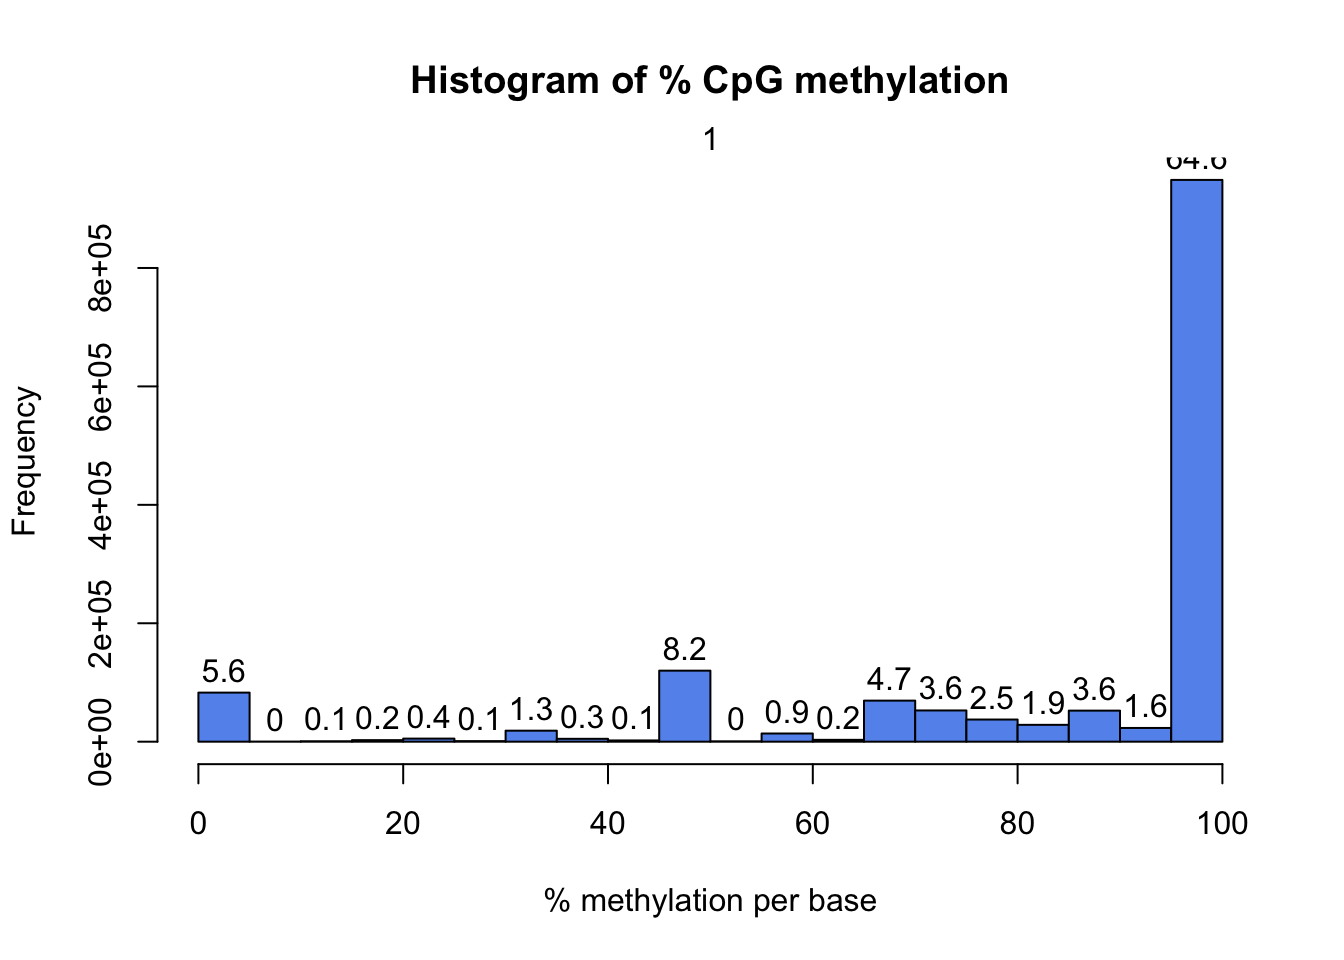
\includegraphics{02-matrices_files/figure-latex/unnamed-chunk-4-1.pdf}
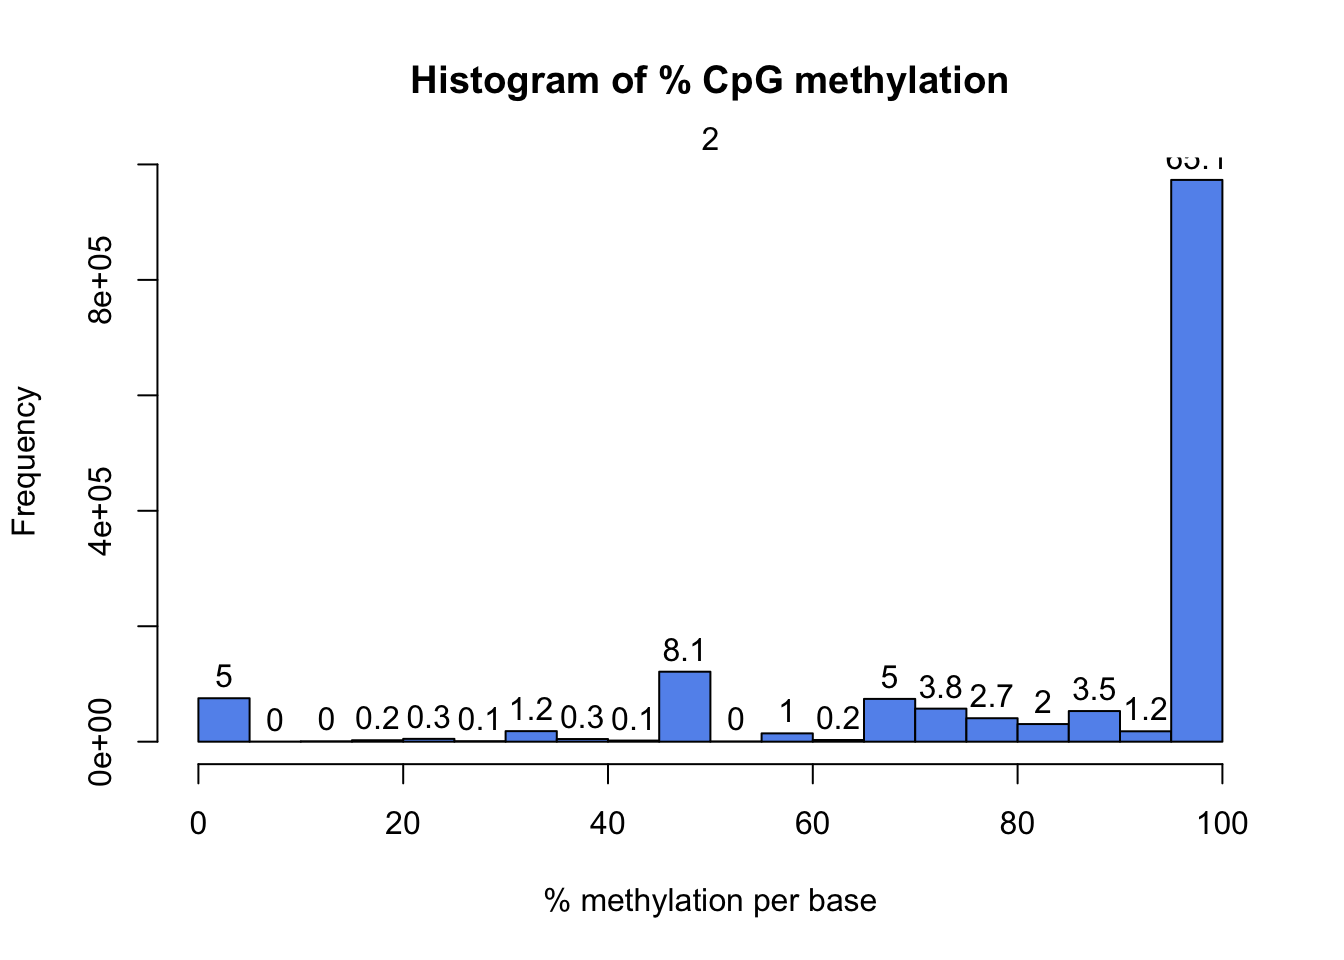
\includegraphics{02-matrices_files/figure-latex/unnamed-chunk-4-2.pdf}
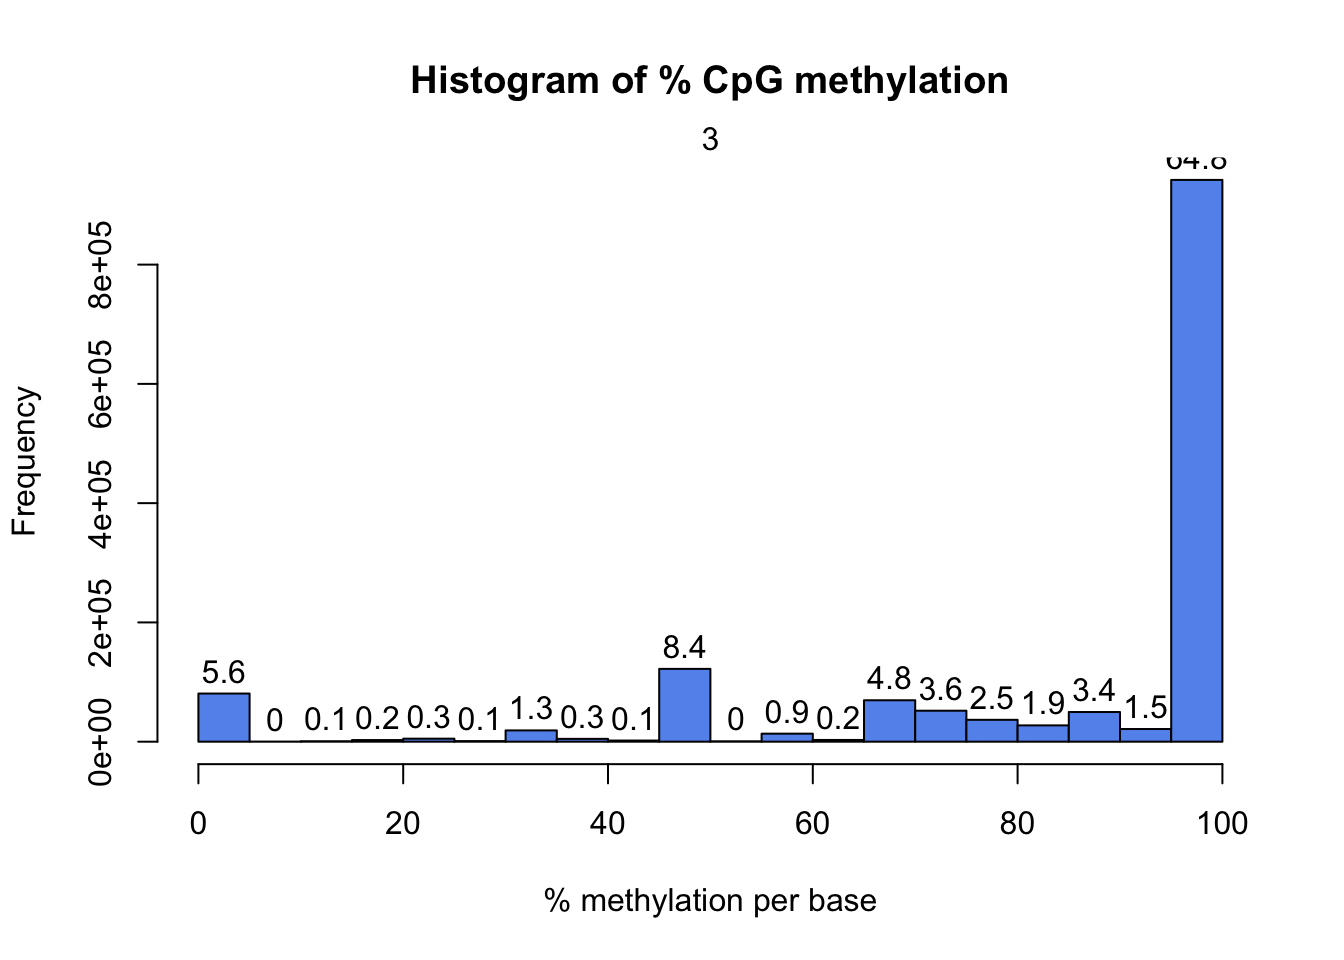
\includegraphics{02-matrices_files/figure-latex/unnamed-chunk-4-3.pdf}
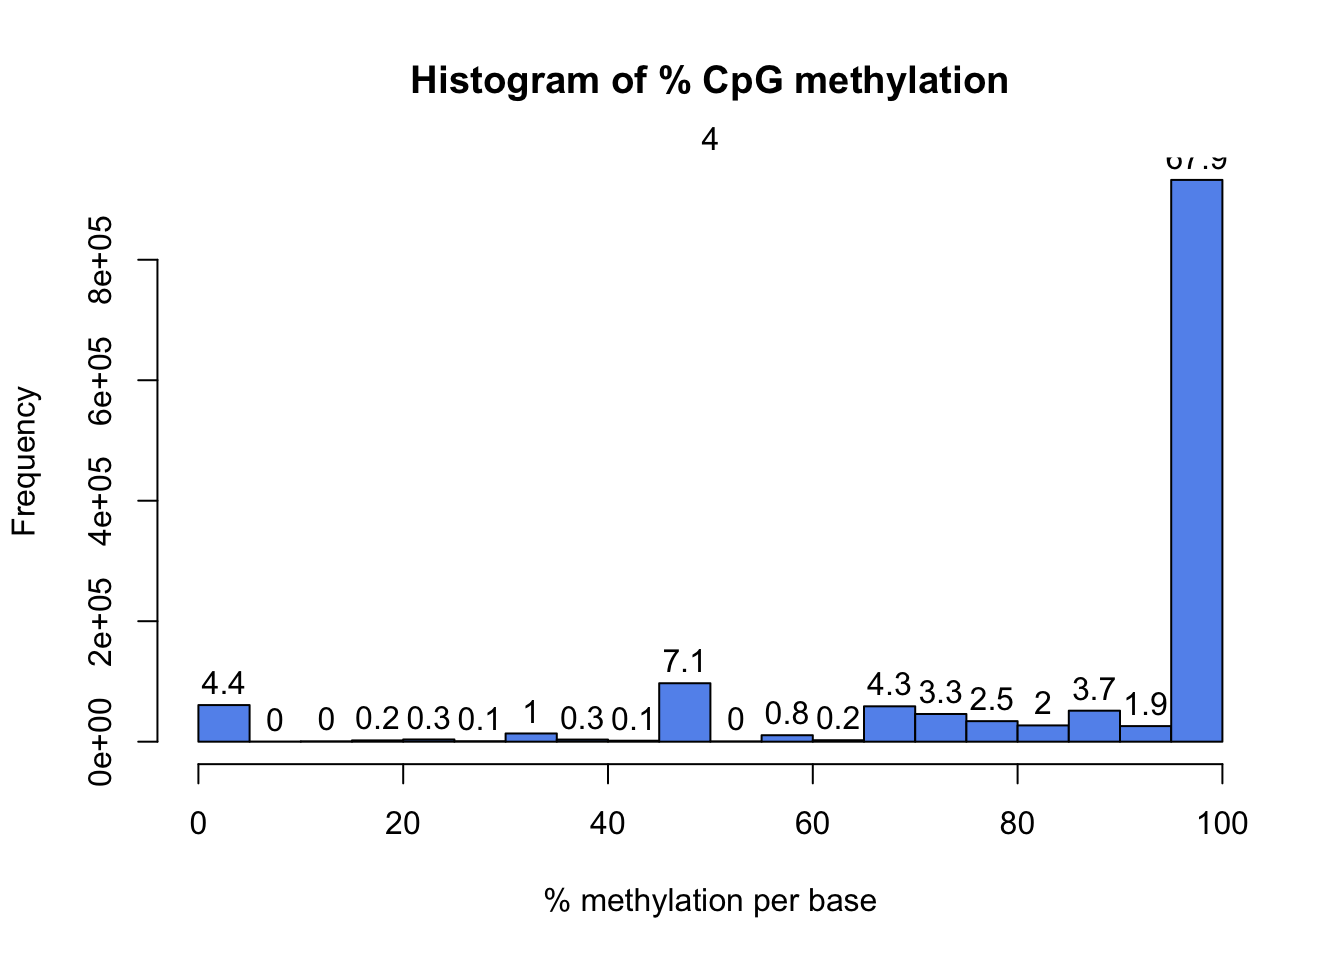
\includegraphics{02-matrices_files/figure-latex/unnamed-chunk-4-4.pdf}
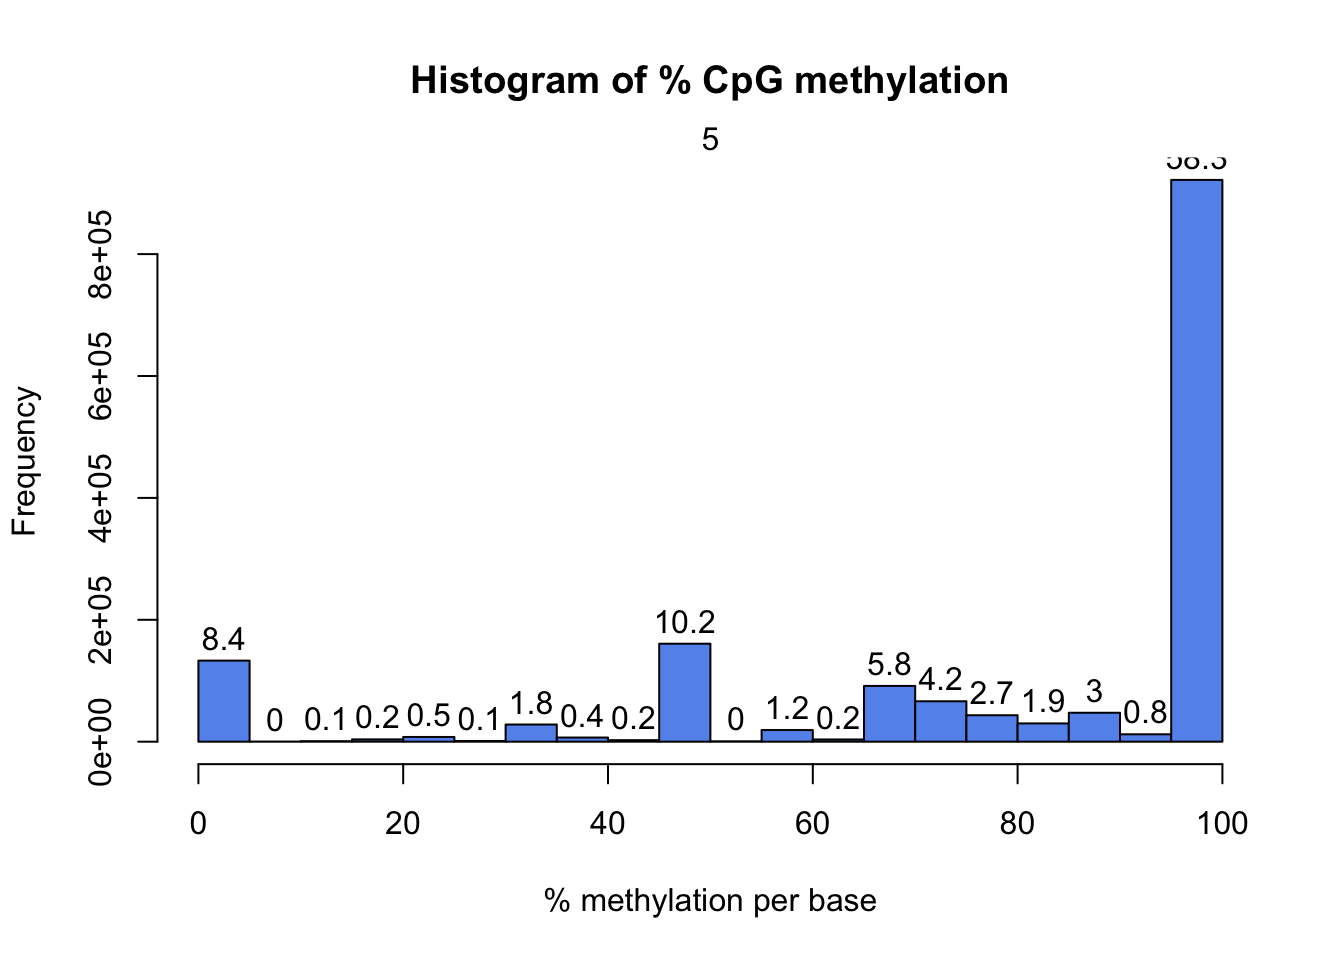
\includegraphics{02-matrices_files/figure-latex/unnamed-chunk-4-5.pdf}
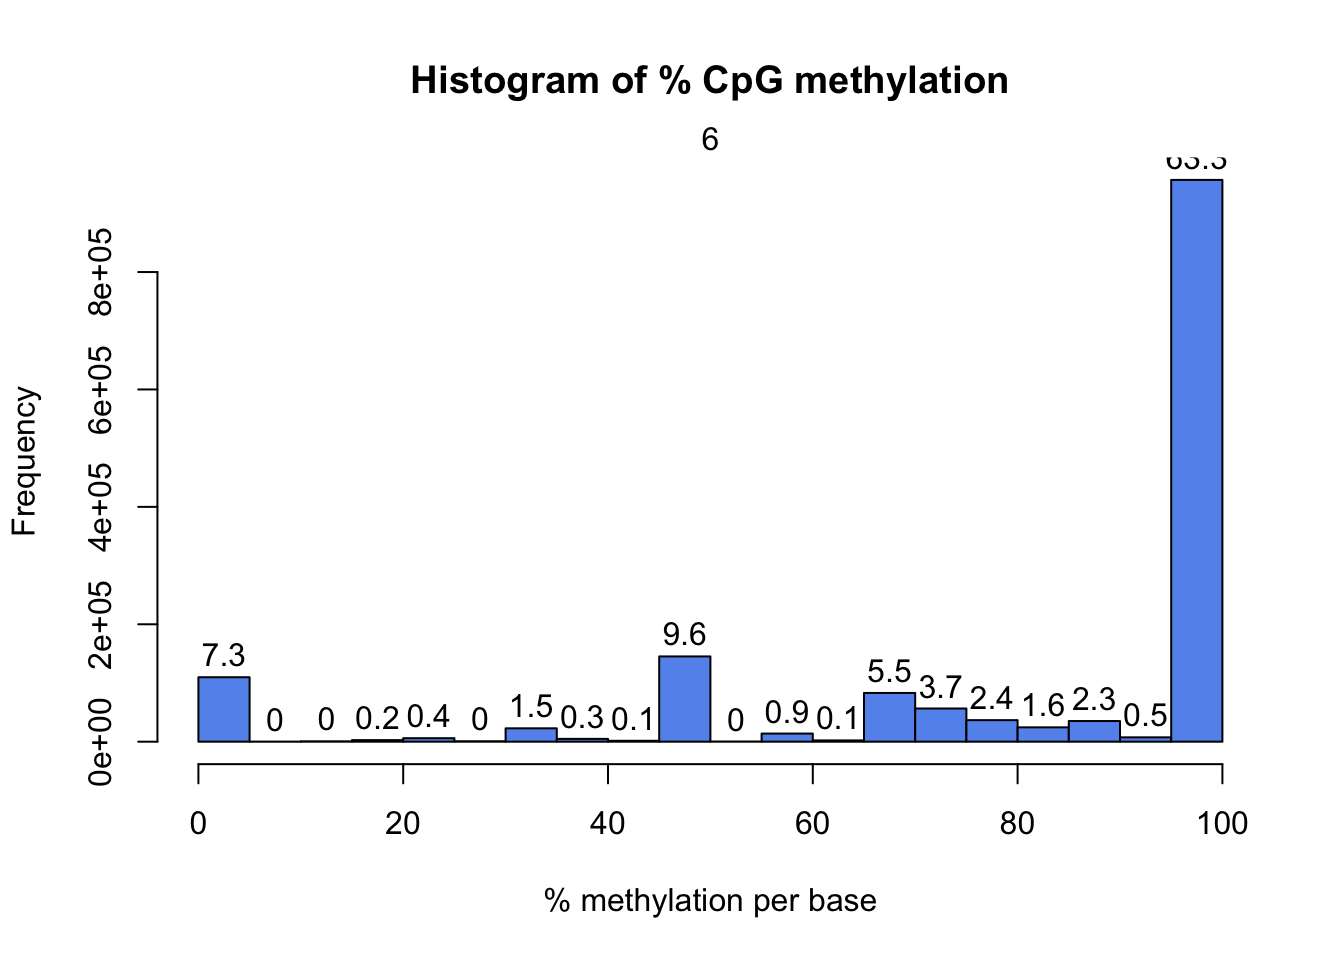
\includegraphics{02-matrices_files/figure-latex/unnamed-chunk-4-6.pdf}
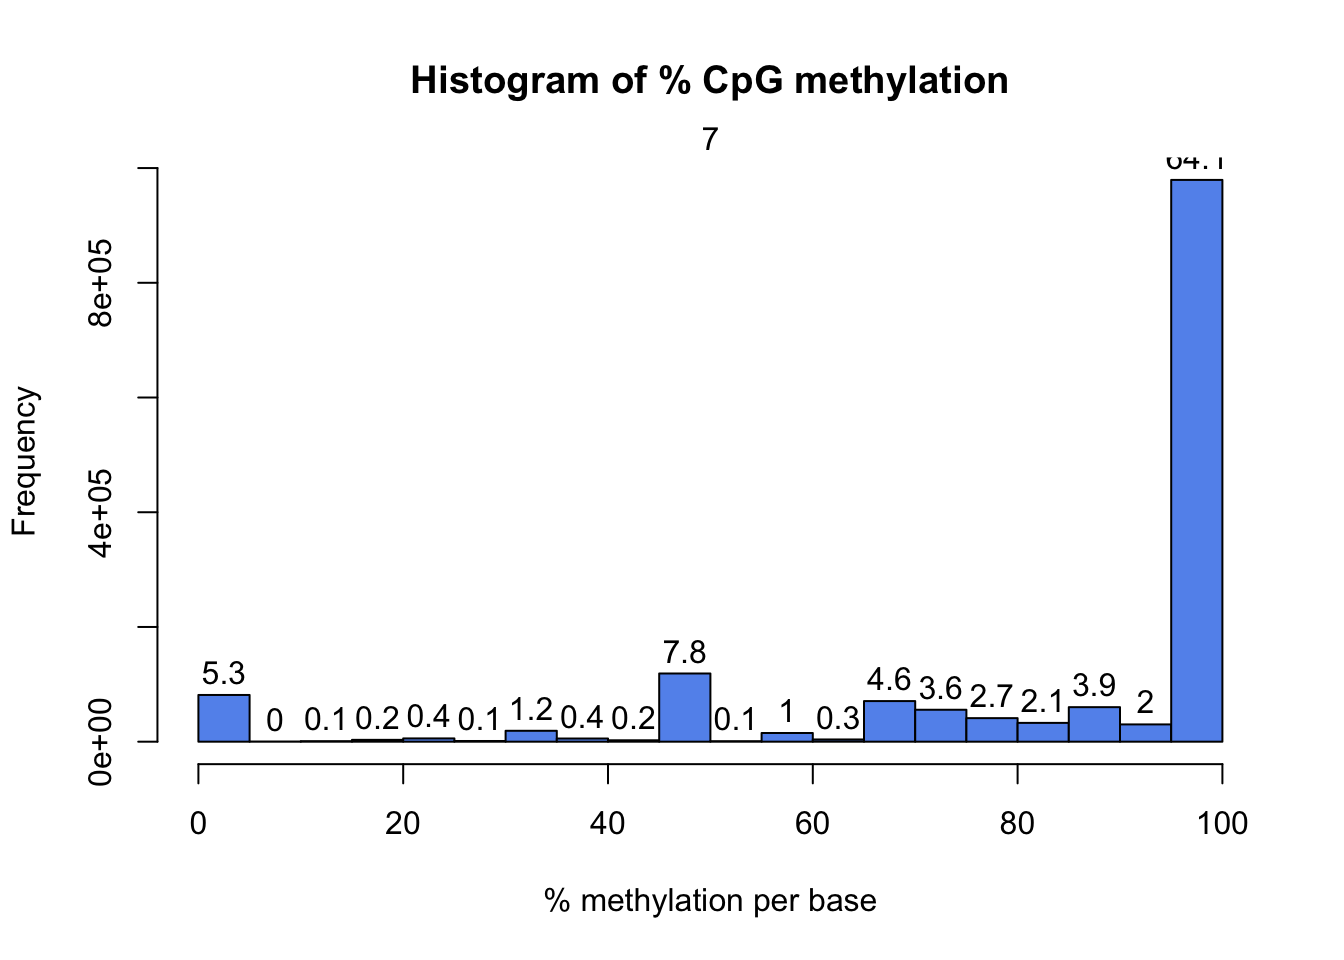
\includegraphics{02-matrices_files/figure-latex/unnamed-chunk-4-7.pdf}
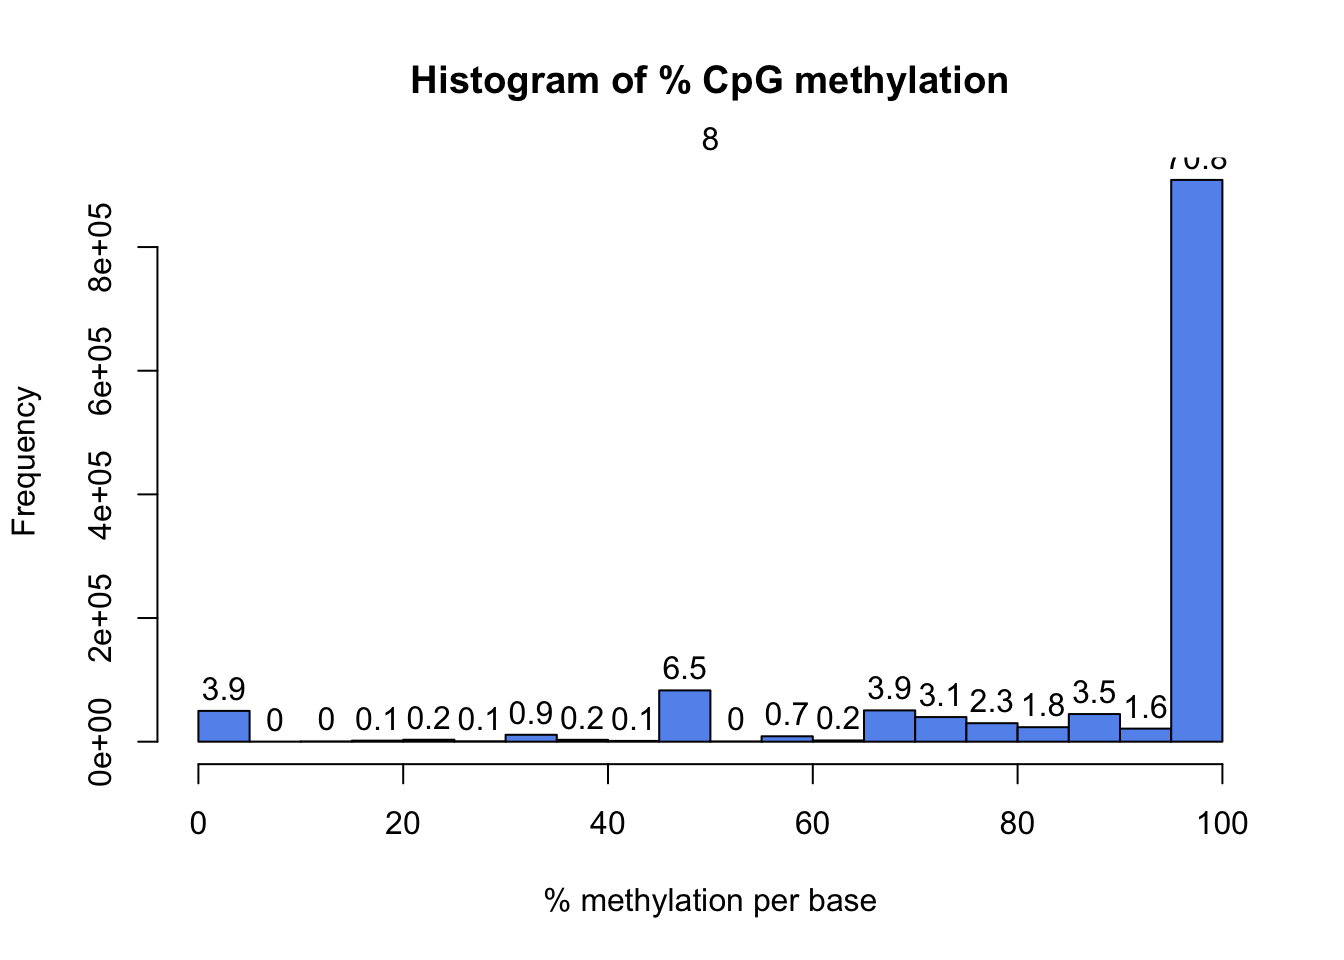
\includegraphics{02-matrices_files/figure-latex/unnamed-chunk-4-8.pdf}
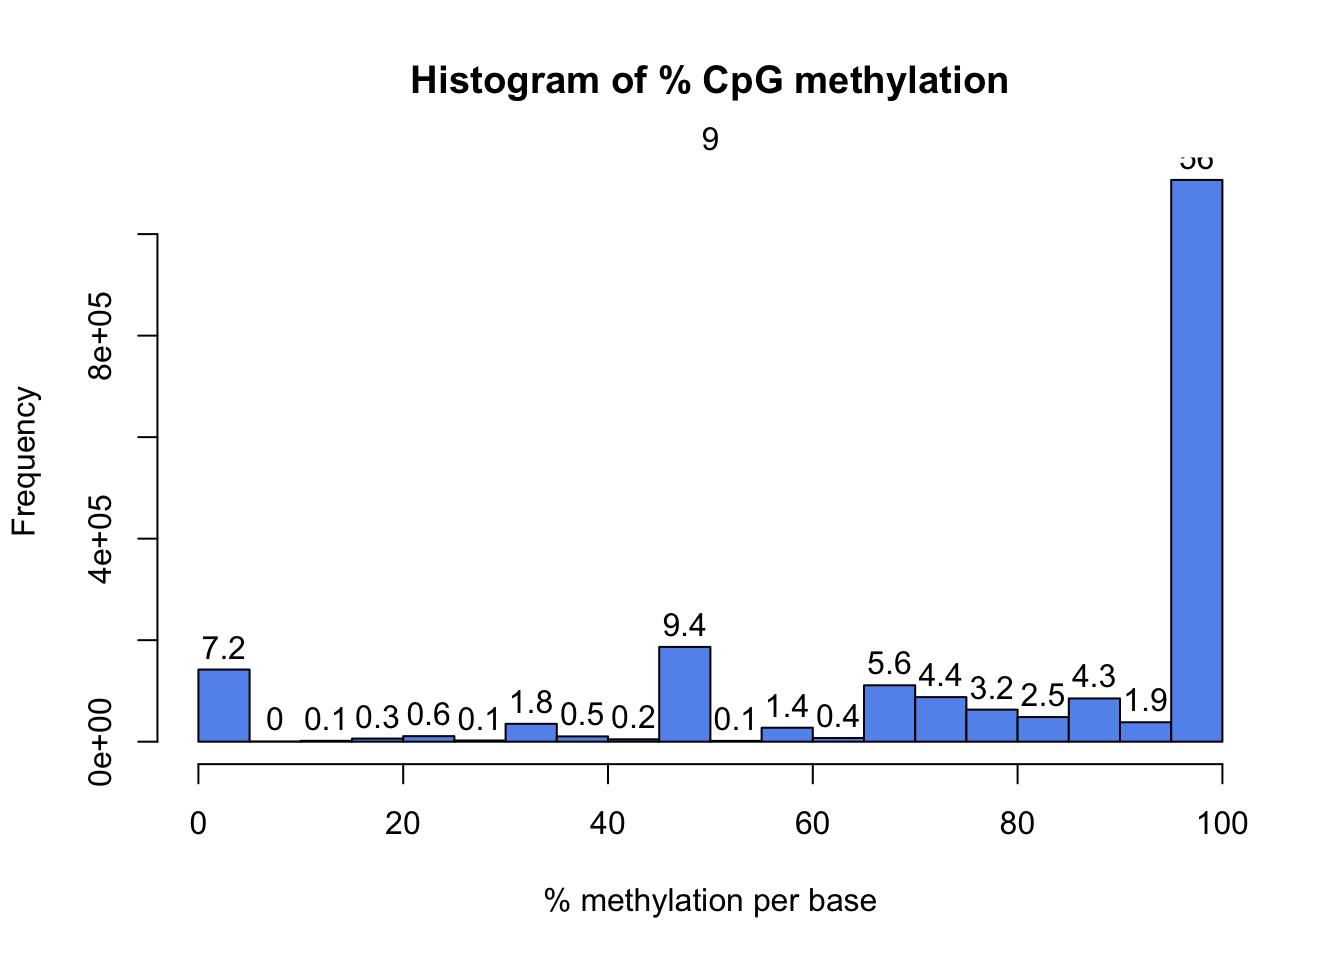
\includegraphics{02-matrices_files/figure-latex/unnamed-chunk-4-9.pdf}
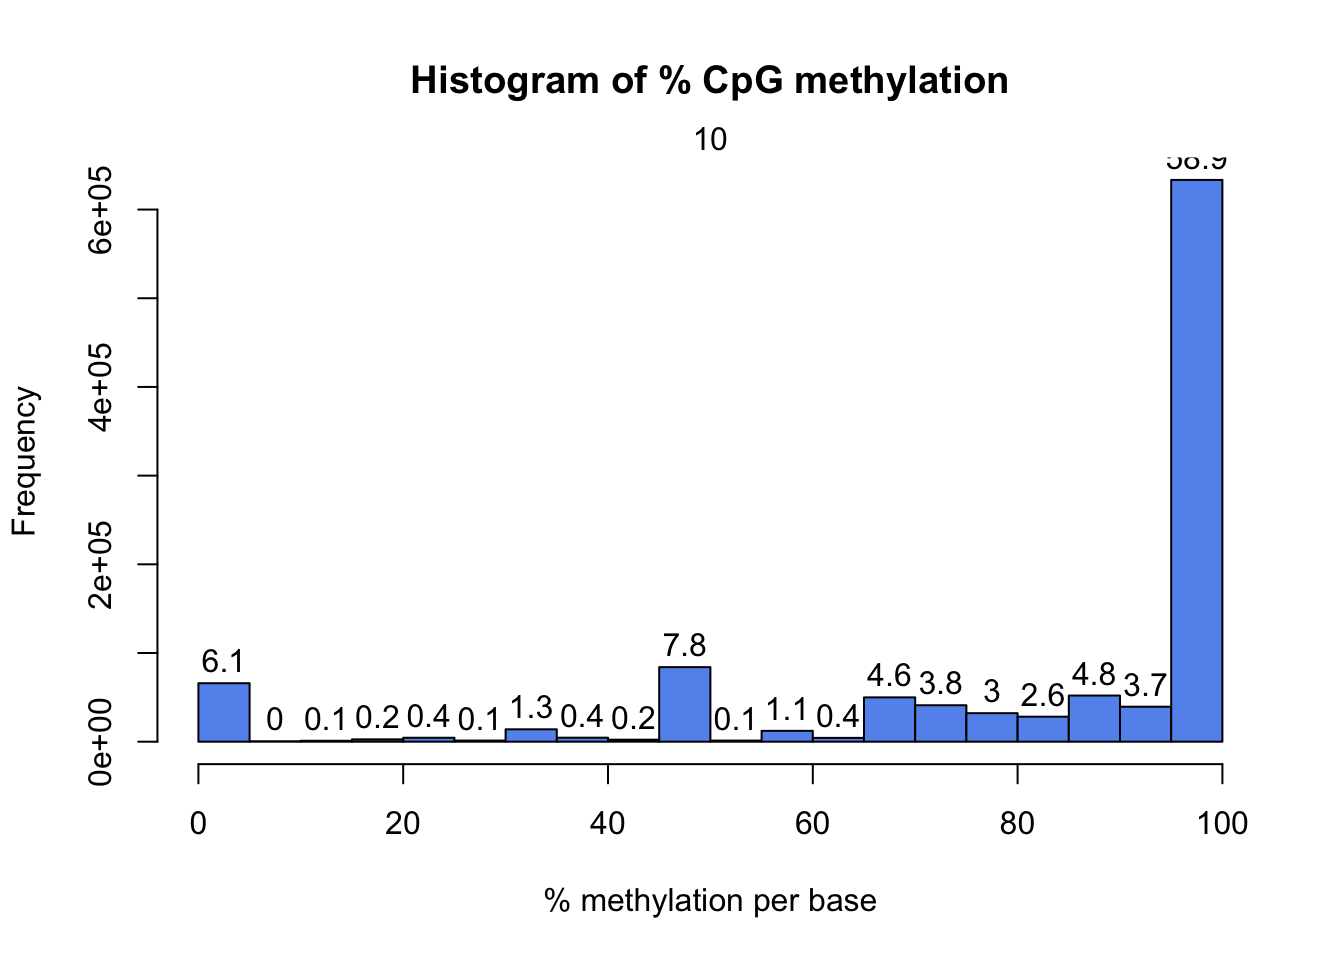
\includegraphics{02-matrices_files/figure-latex/unnamed-chunk-4-10.pdf}
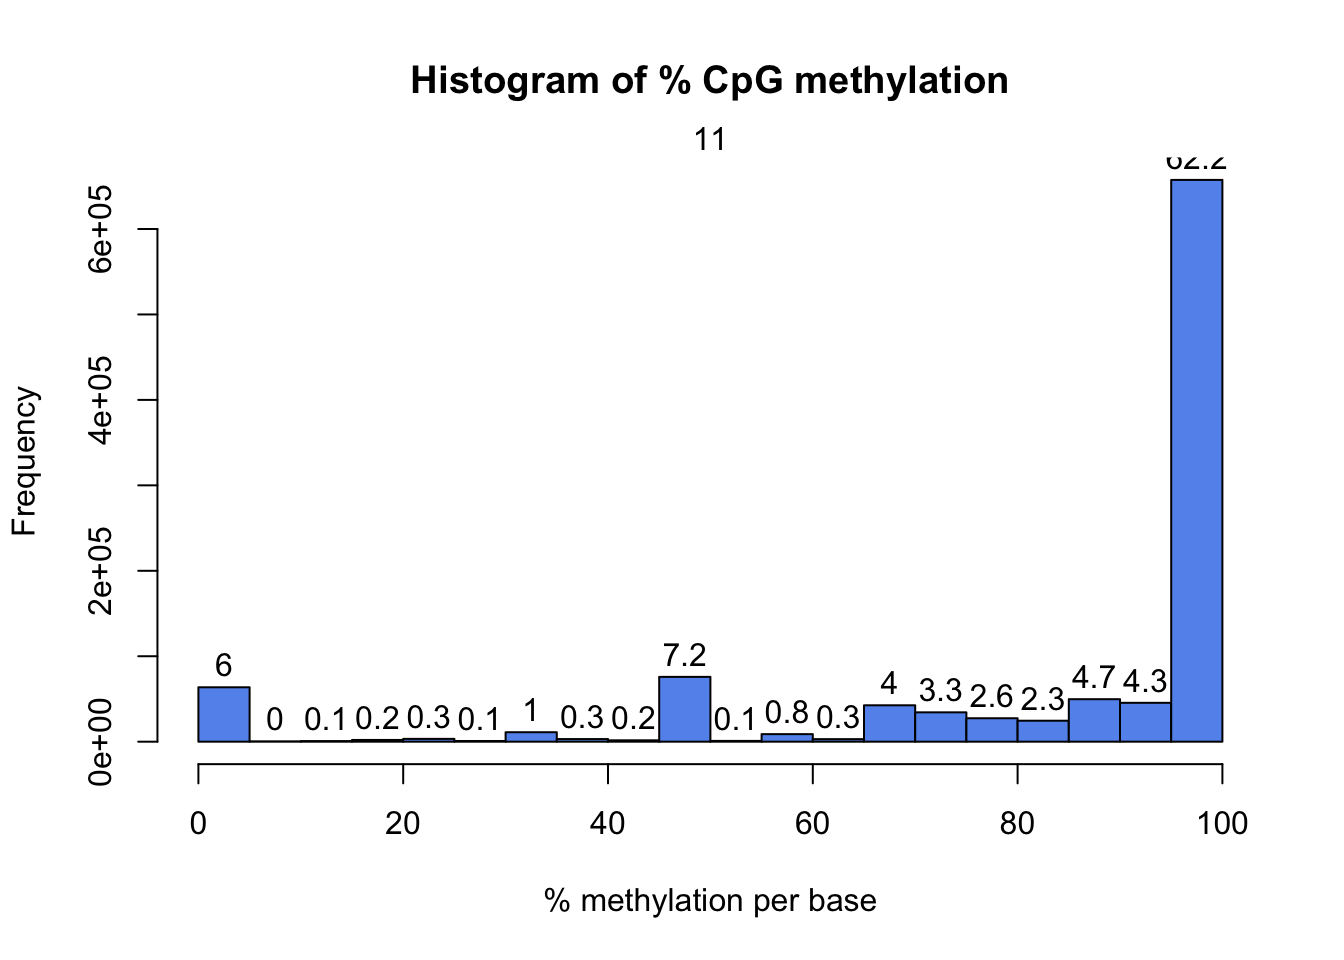
\includegraphics{02-matrices_files/figure-latex/unnamed-chunk-4-11.pdf}
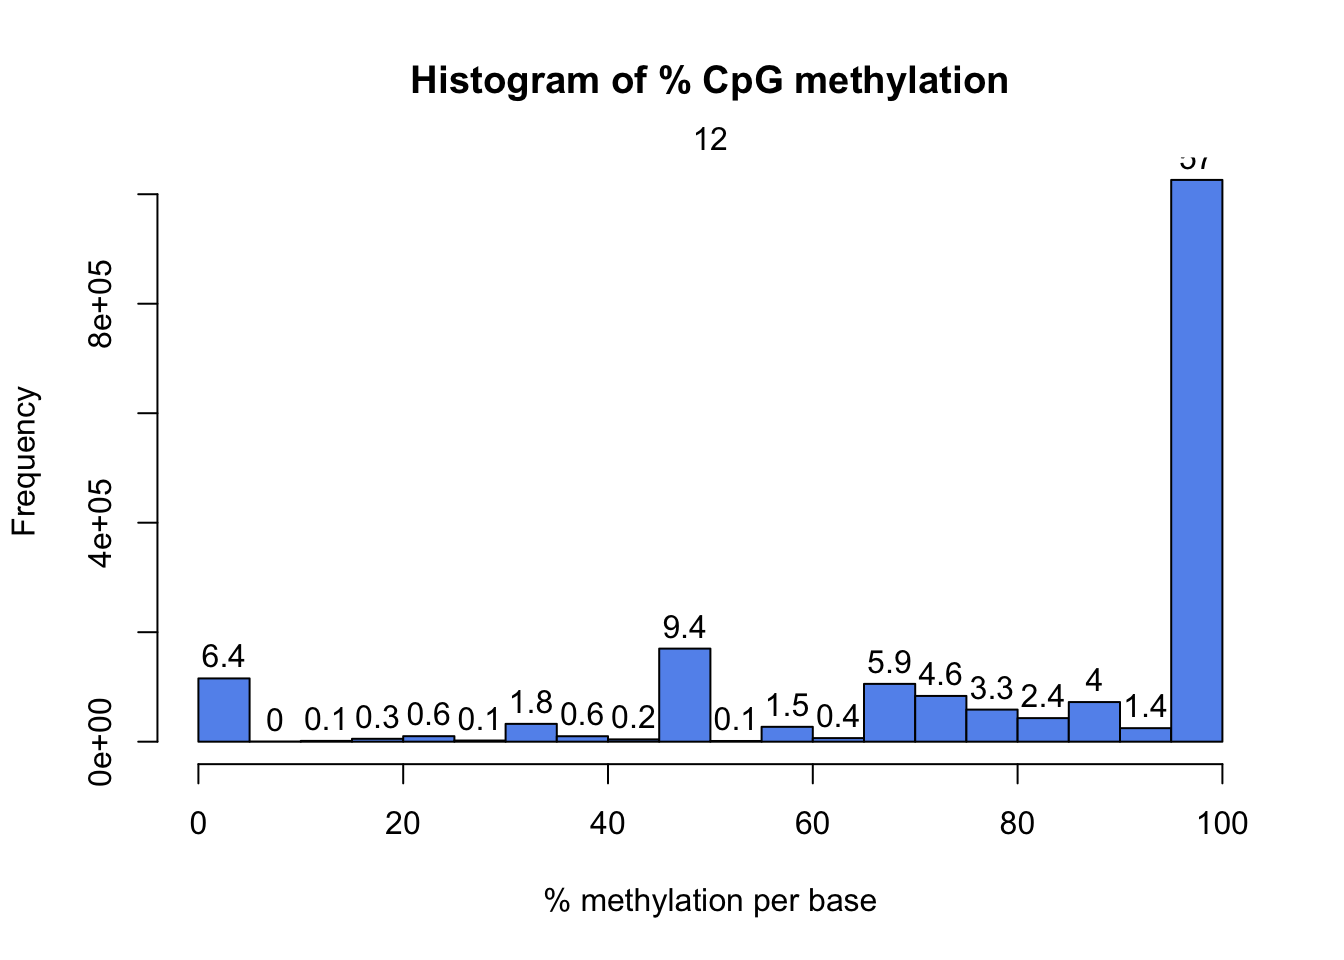
\includegraphics{02-matrices_files/figure-latex/unnamed-chunk-4-12.pdf}
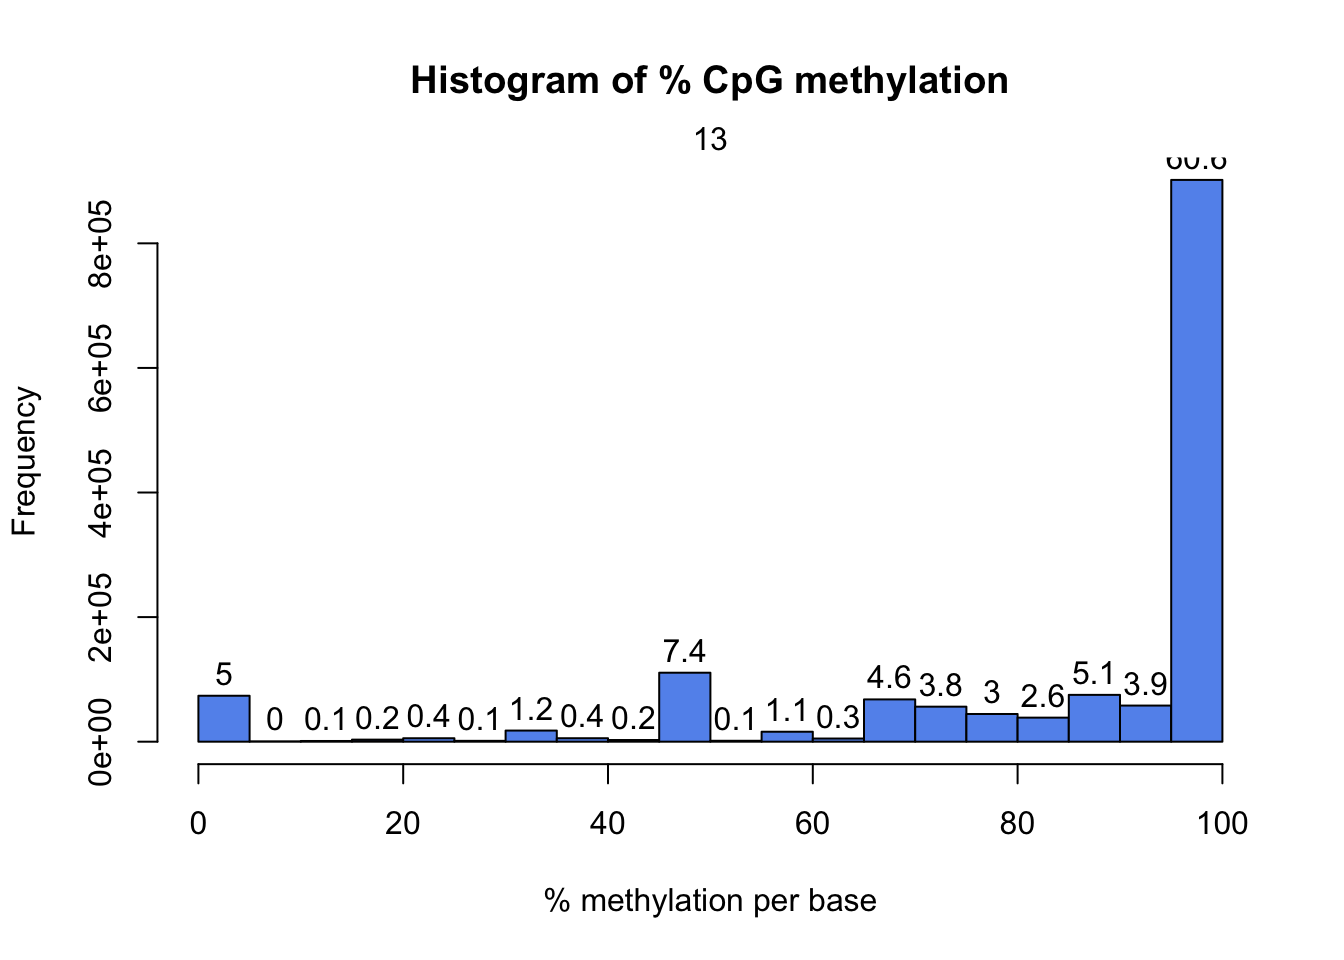
\includegraphics{02-matrices_files/figure-latex/unnamed-chunk-4-13.pdf}
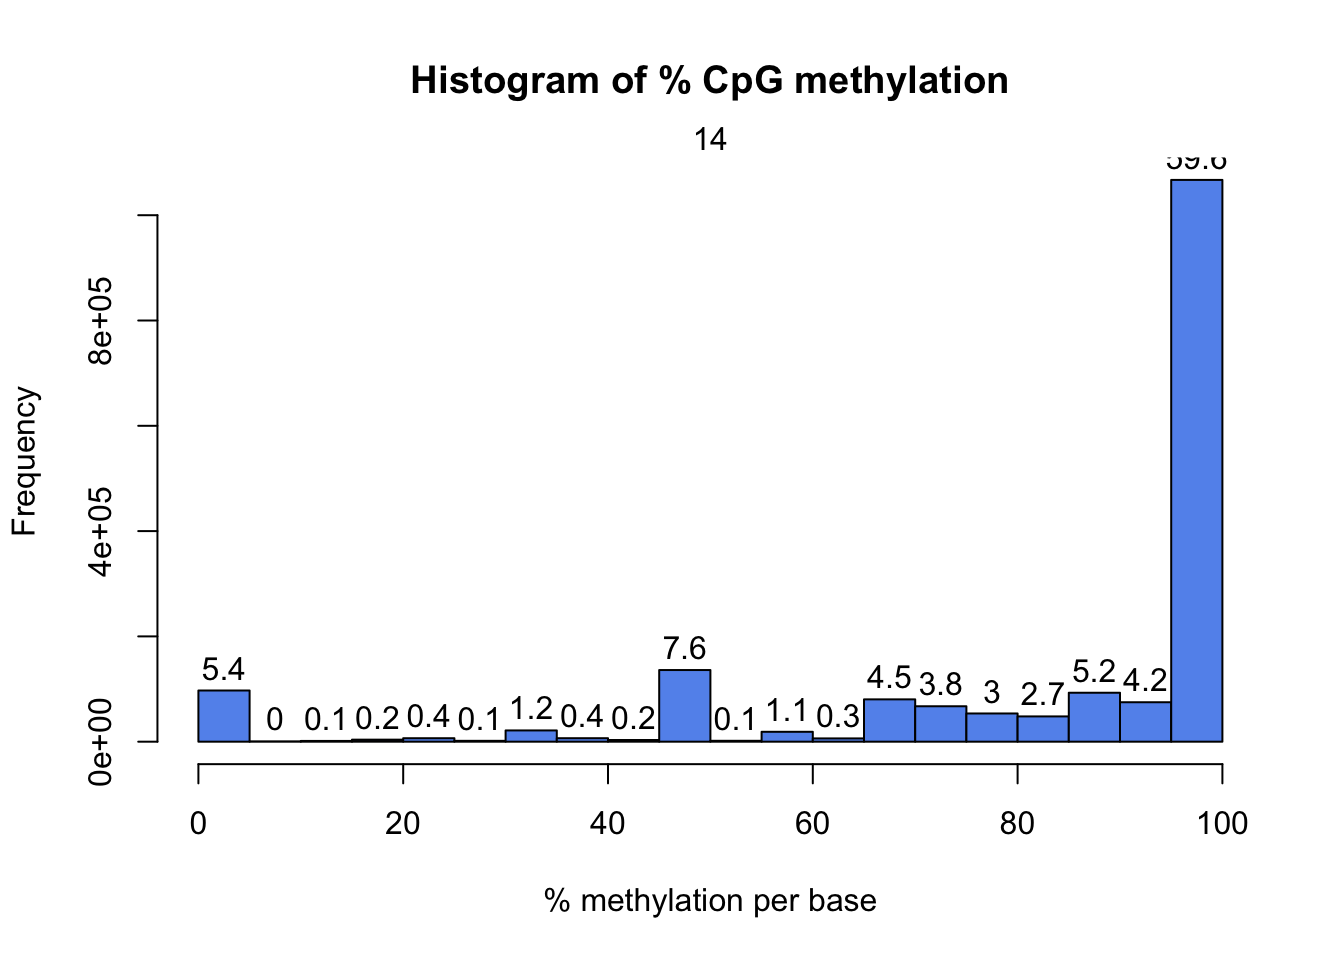
\includegraphics{02-matrices_files/figure-latex/unnamed-chunk-4-14.pdf}
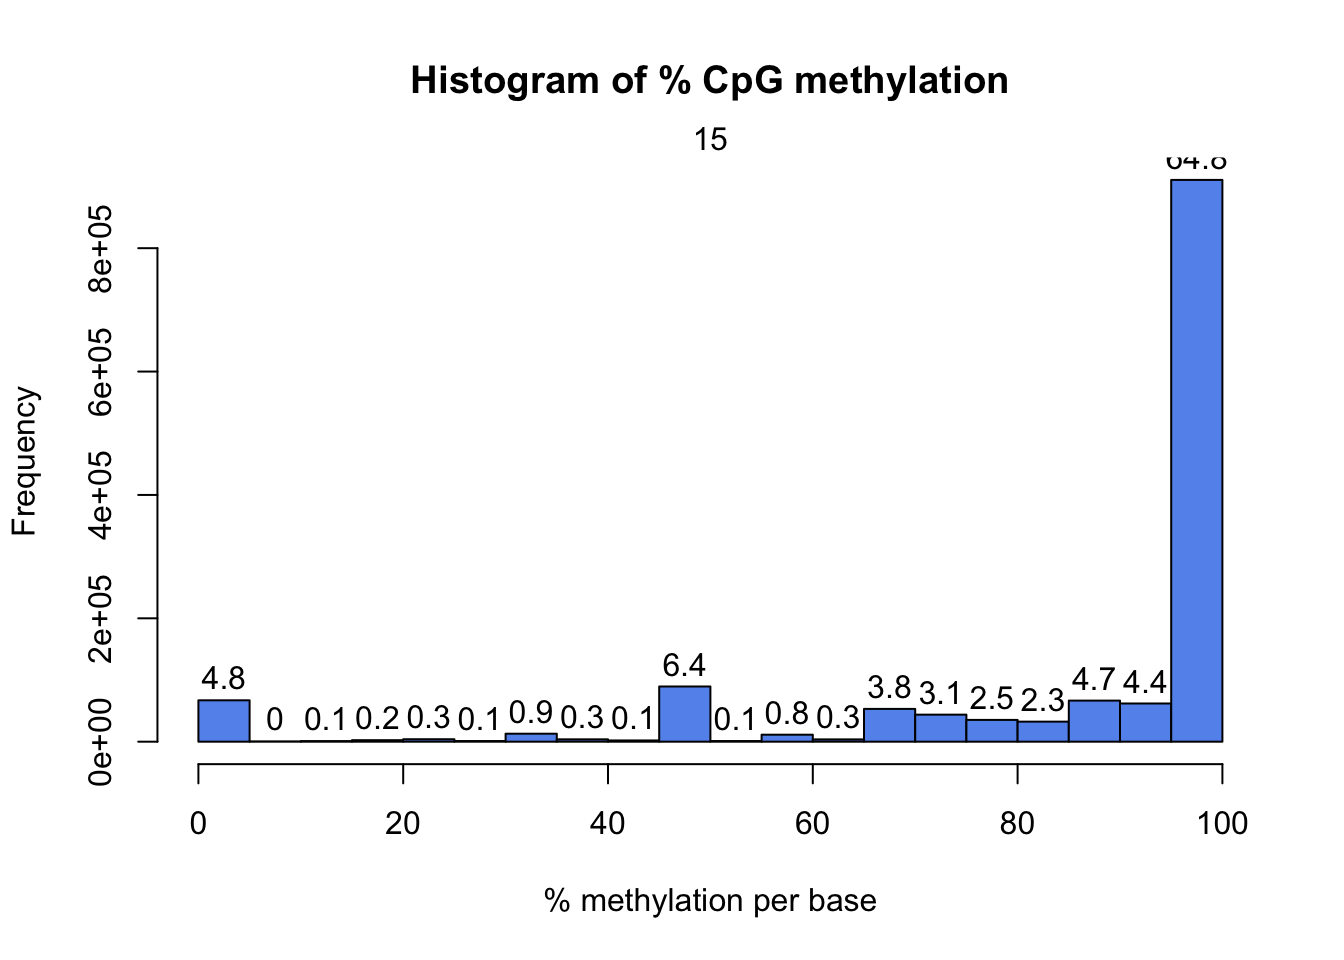
\includegraphics{02-matrices_files/figure-latex/unnamed-chunk-4-15.pdf}
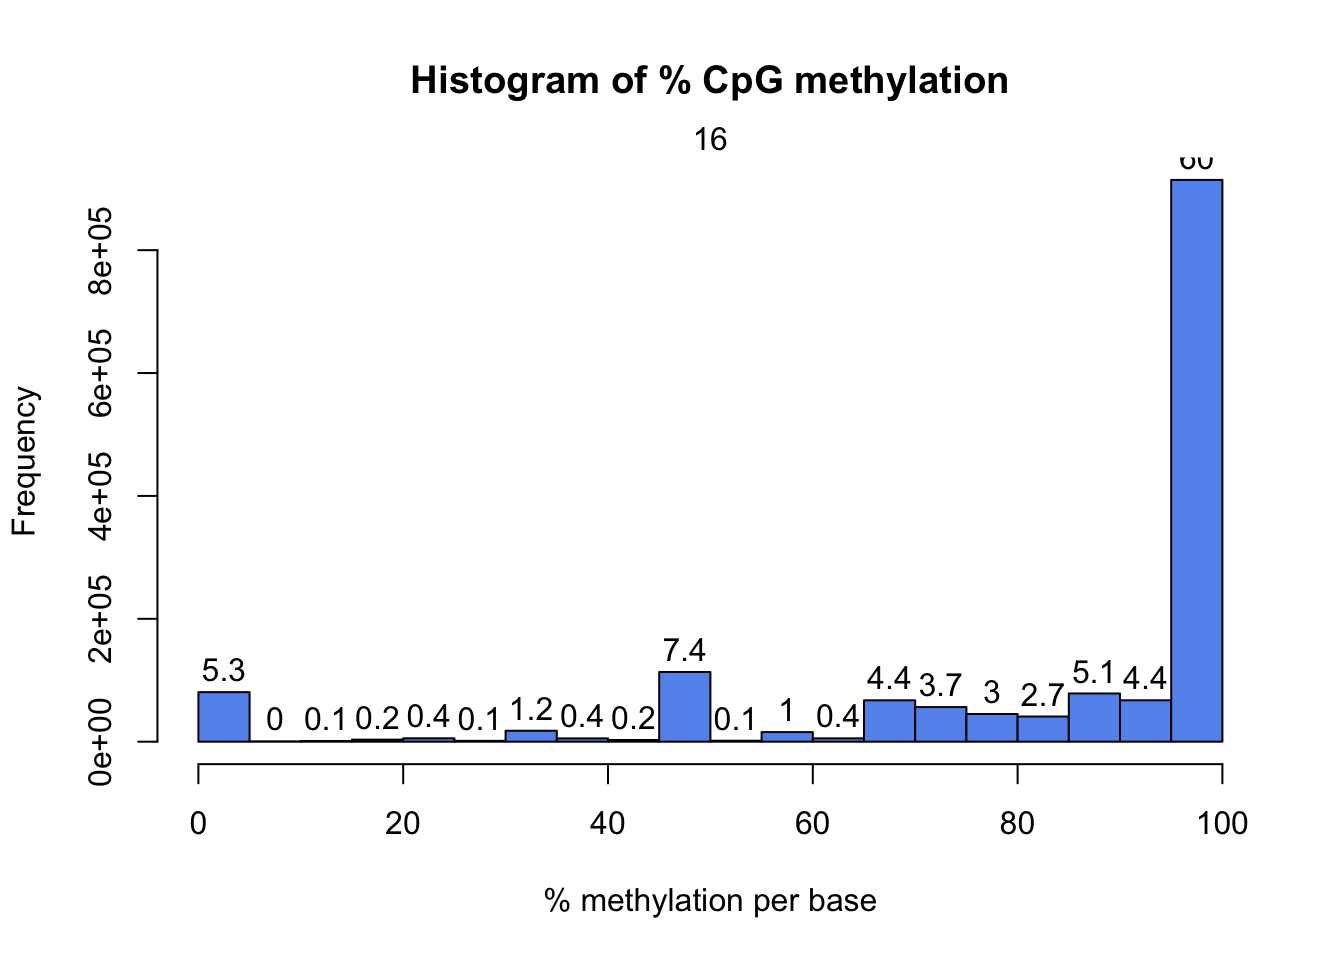
\includegraphics{02-matrices_files/figure-latex/unnamed-chunk-4-16.pdf}
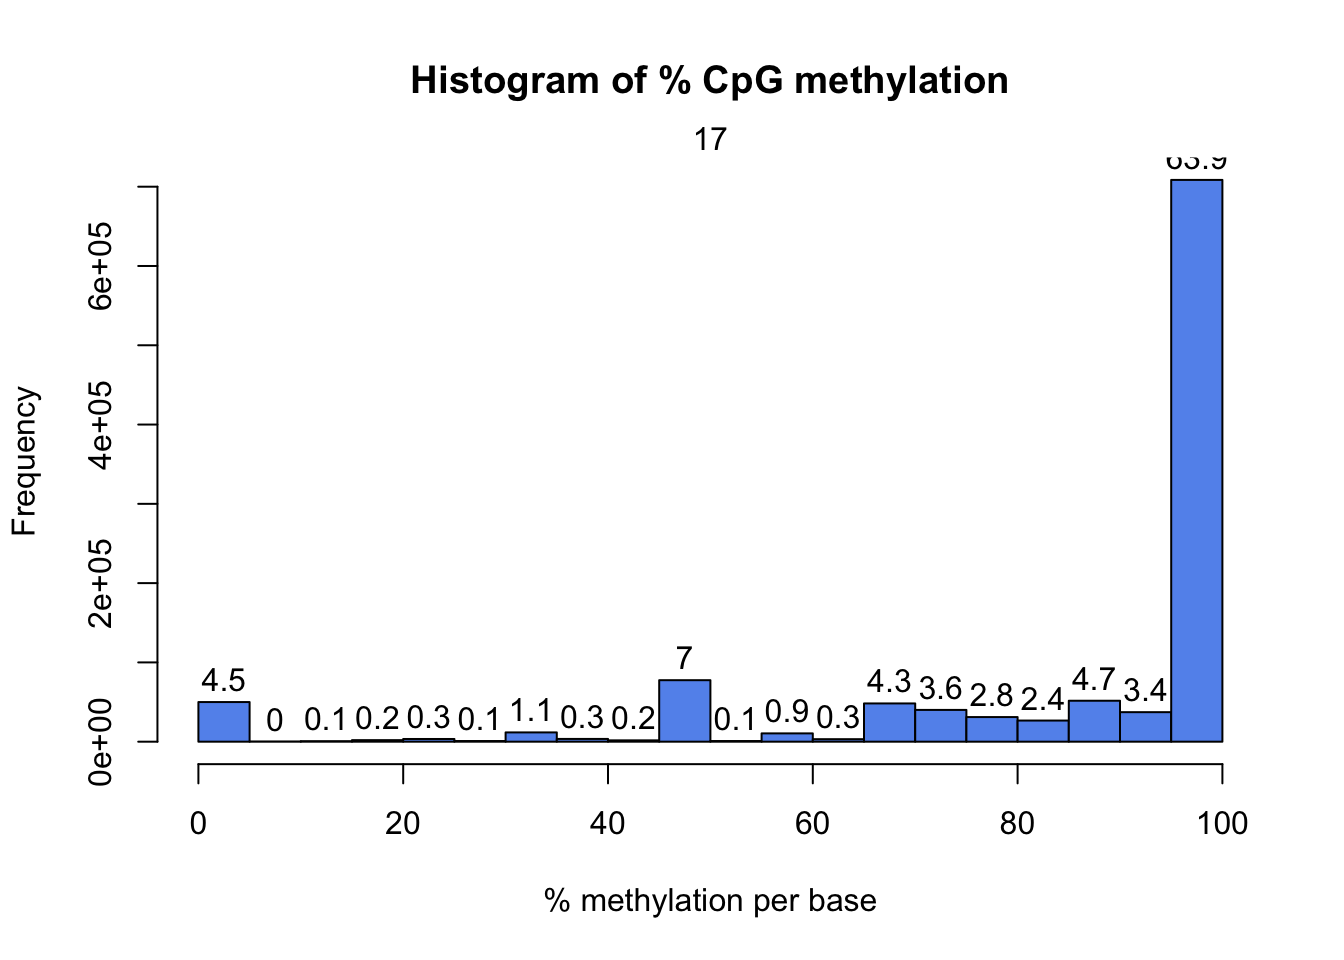
\includegraphics{02-matrices_files/figure-latex/unnamed-chunk-4-17.pdf}
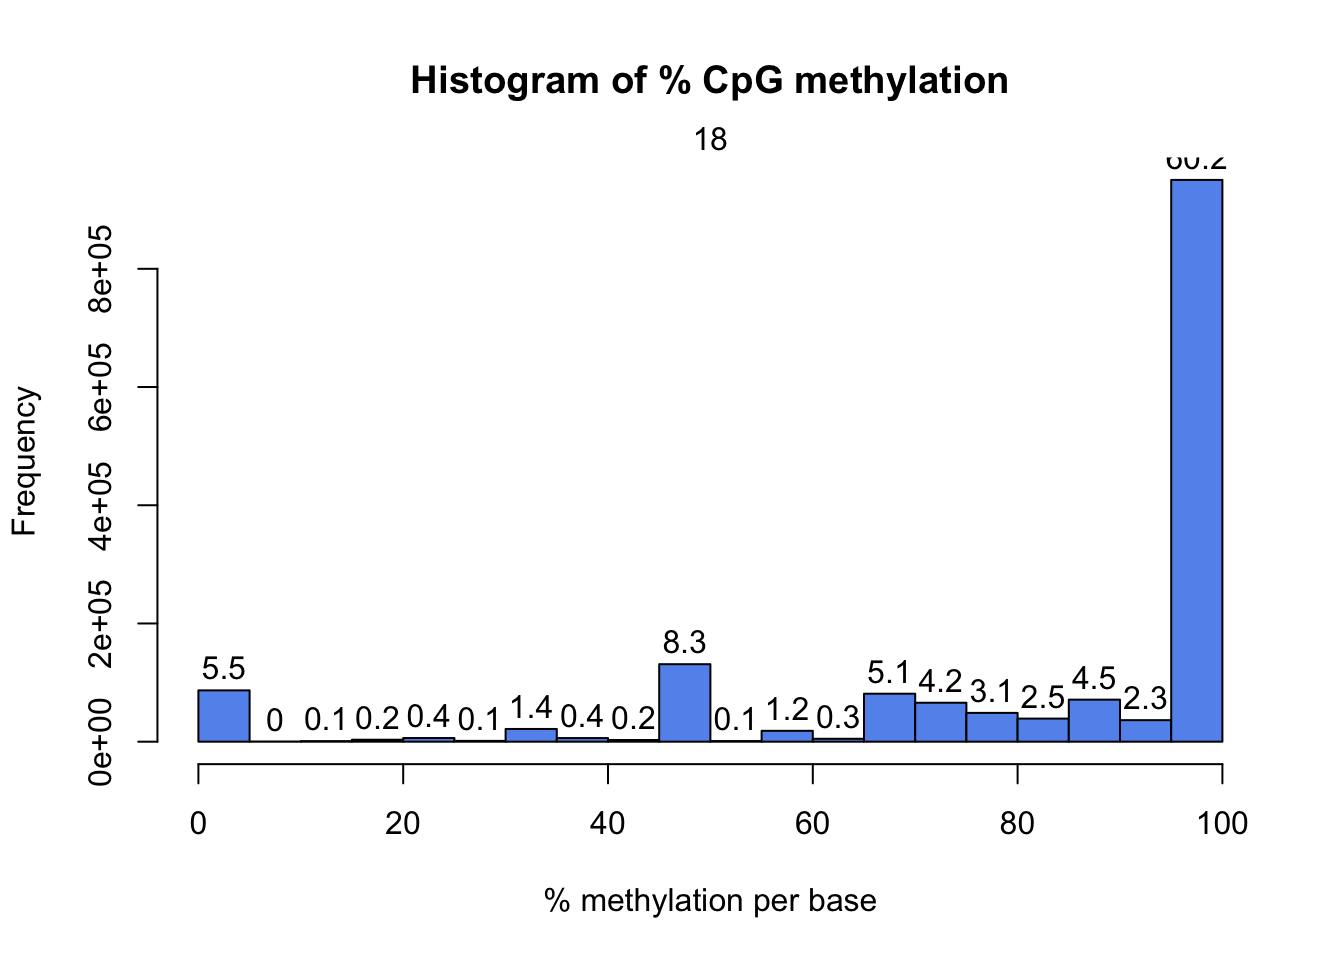
\includegraphics{02-matrices_files/figure-latex/unnamed-chunk-4-18.pdf}

We can also plot the read coverage per base information in a similar
way, again numbers on bars denote what percentage of locations are
contained in that bin. Experiments that are highly suffering from PCR
duplication bias will have a secondary peak towards the right hand side
of the histogram.

\begin{Shaded}
\begin{Highlighting}[]
\ControlFlowTok{for}\NormalTok{ (i }\ControlFlowTok{in} \DecValTok{1}\OperatorTok{:}\DecValTok{18}\NormalTok{) \{}
  \KeywordTok{getCoverageStats}\NormalTok{(myobj_}\DecValTok{18}\NormalTok{[[i]],}\DataTypeTok{plot=}\OtherTok{TRUE}\NormalTok{,}\DataTypeTok{both.strands=}\OtherTok{FALSE}\NormalTok{)}
\NormalTok{\}}
\end{Highlighting}
\end{Shaded}

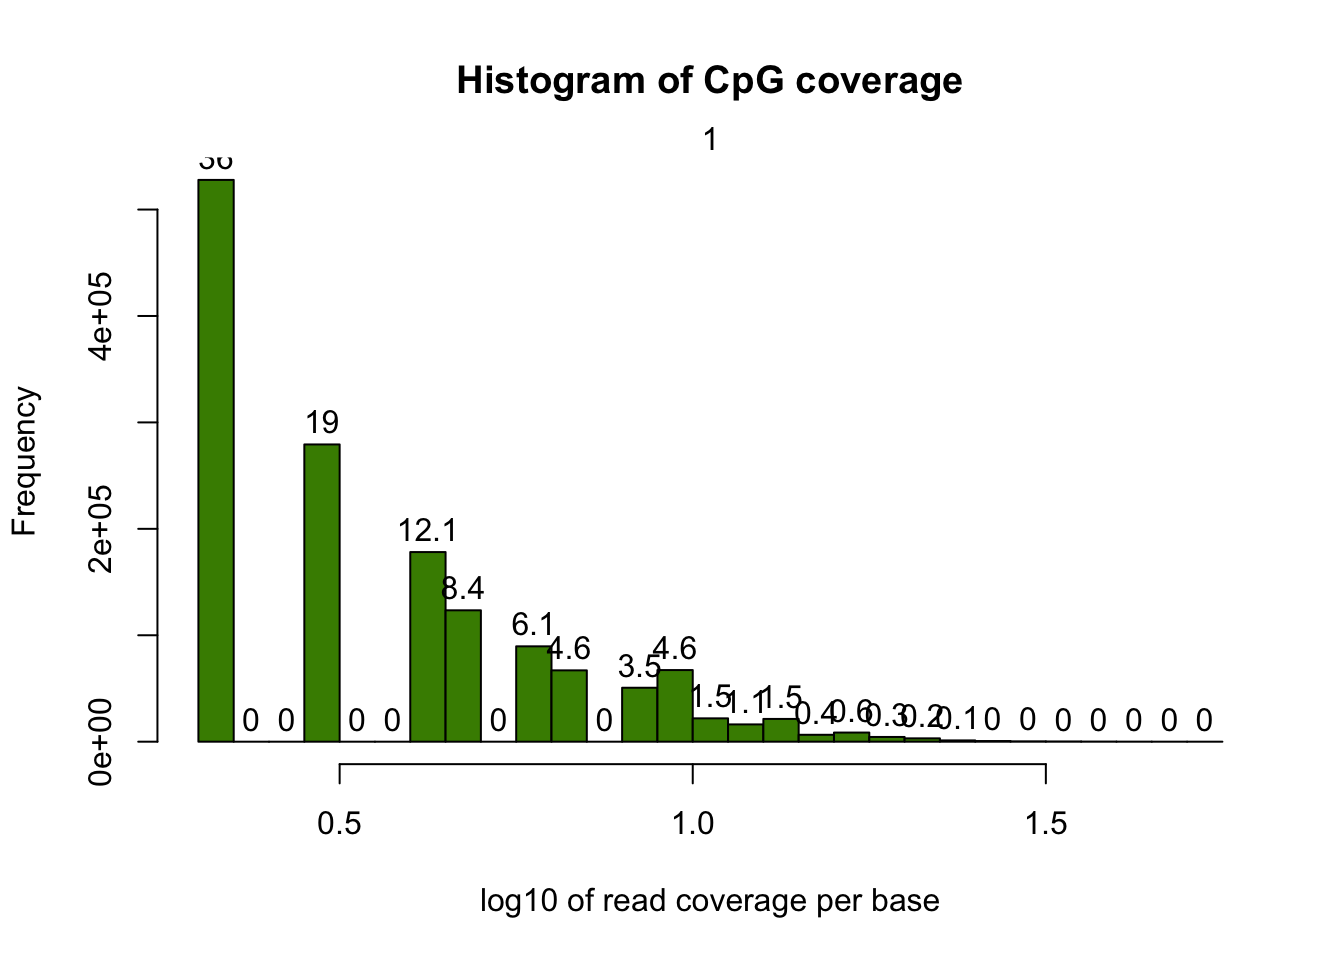
\includegraphics{02-matrices_files/figure-latex/unnamed-chunk-5-1.pdf}
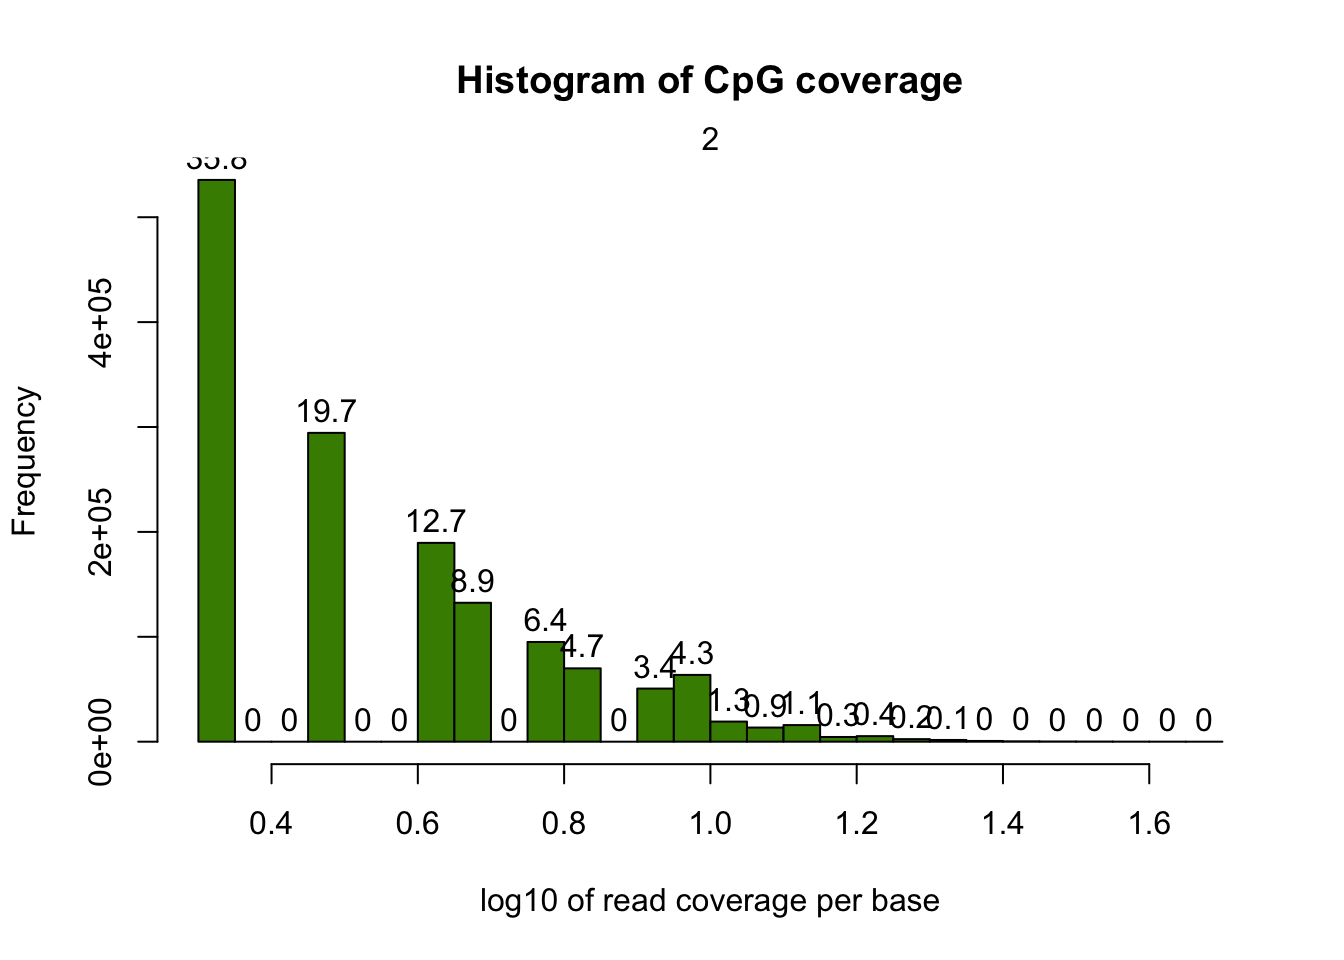
\includegraphics{02-matrices_files/figure-latex/unnamed-chunk-5-2.pdf}
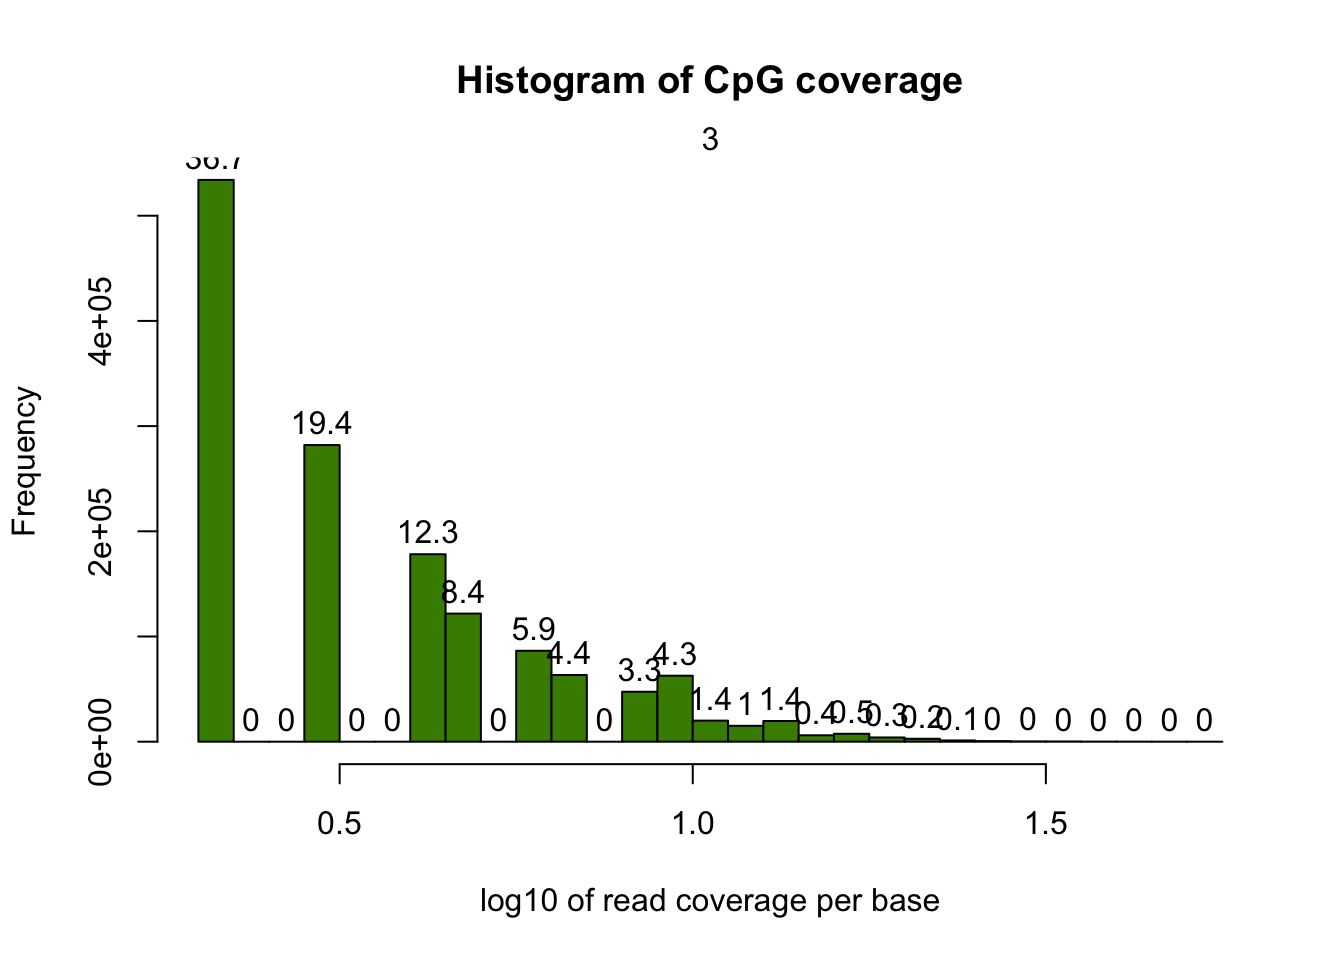
\includegraphics{02-matrices_files/figure-latex/unnamed-chunk-5-3.pdf}
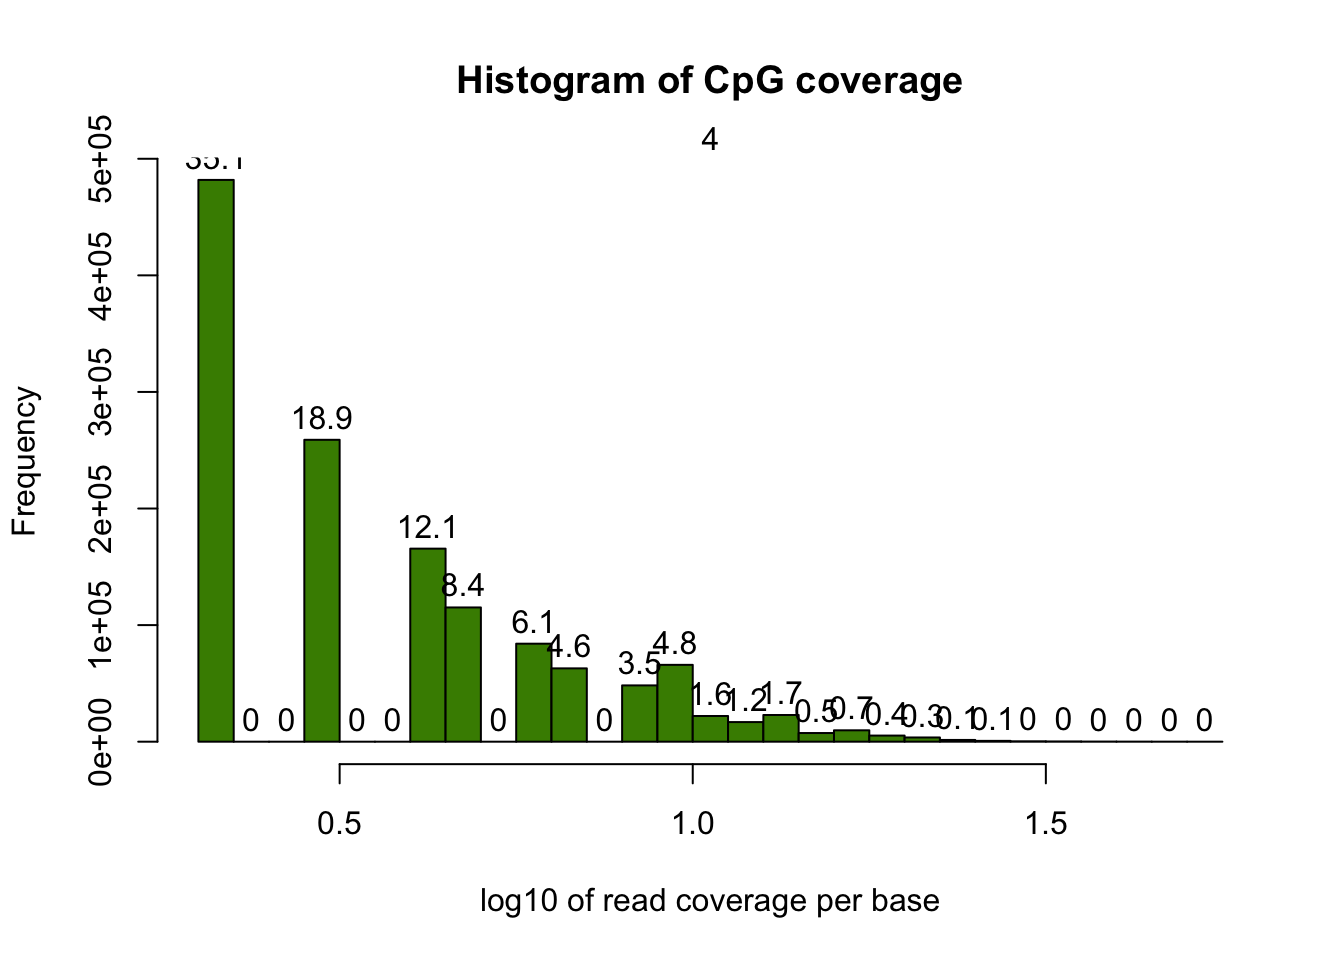
\includegraphics{02-matrices_files/figure-latex/unnamed-chunk-5-4.pdf}
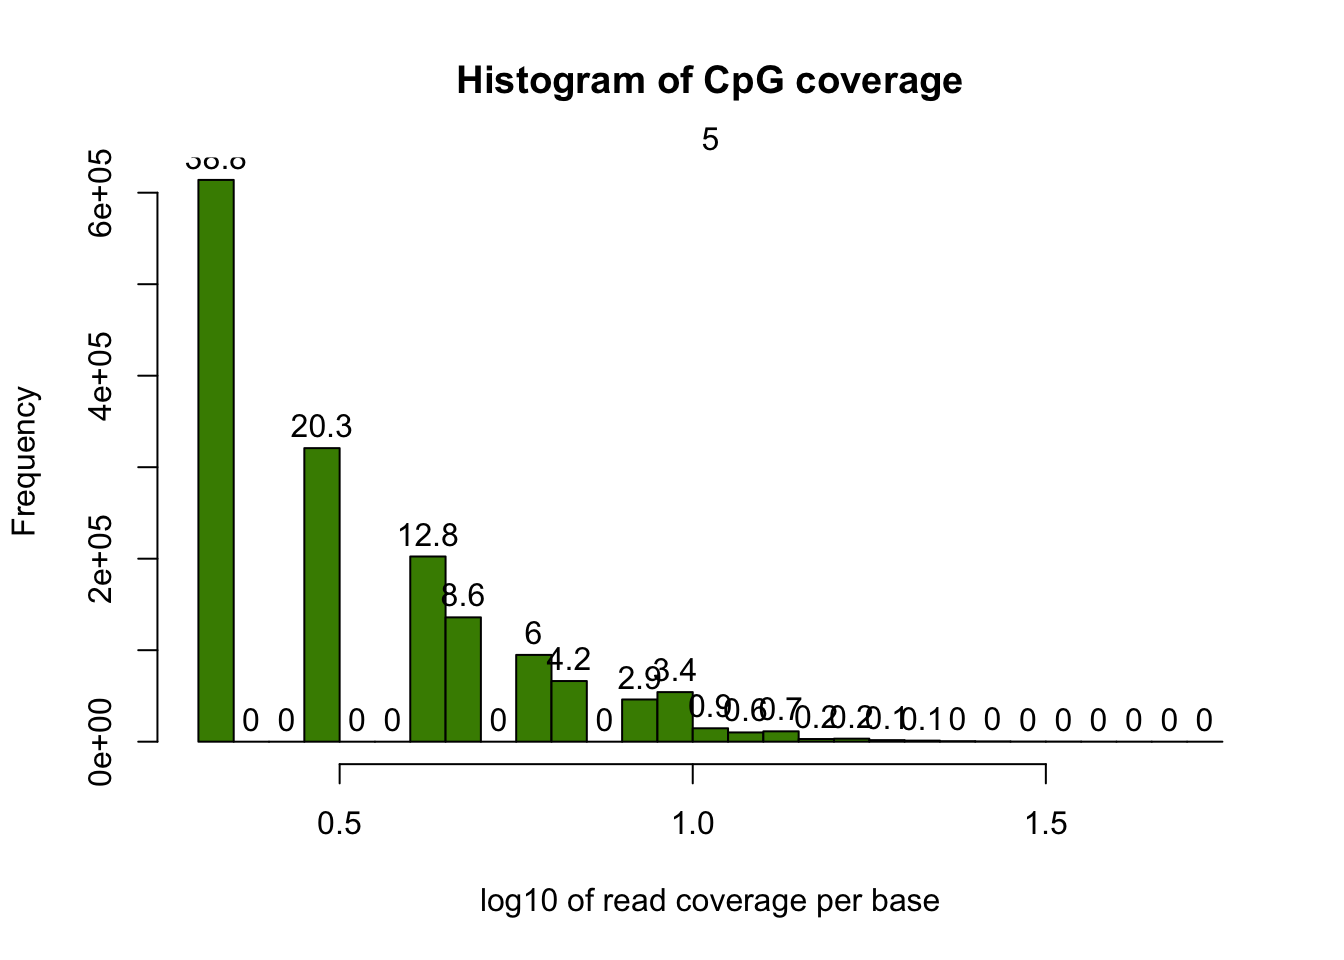
\includegraphics{02-matrices_files/figure-latex/unnamed-chunk-5-5.pdf}
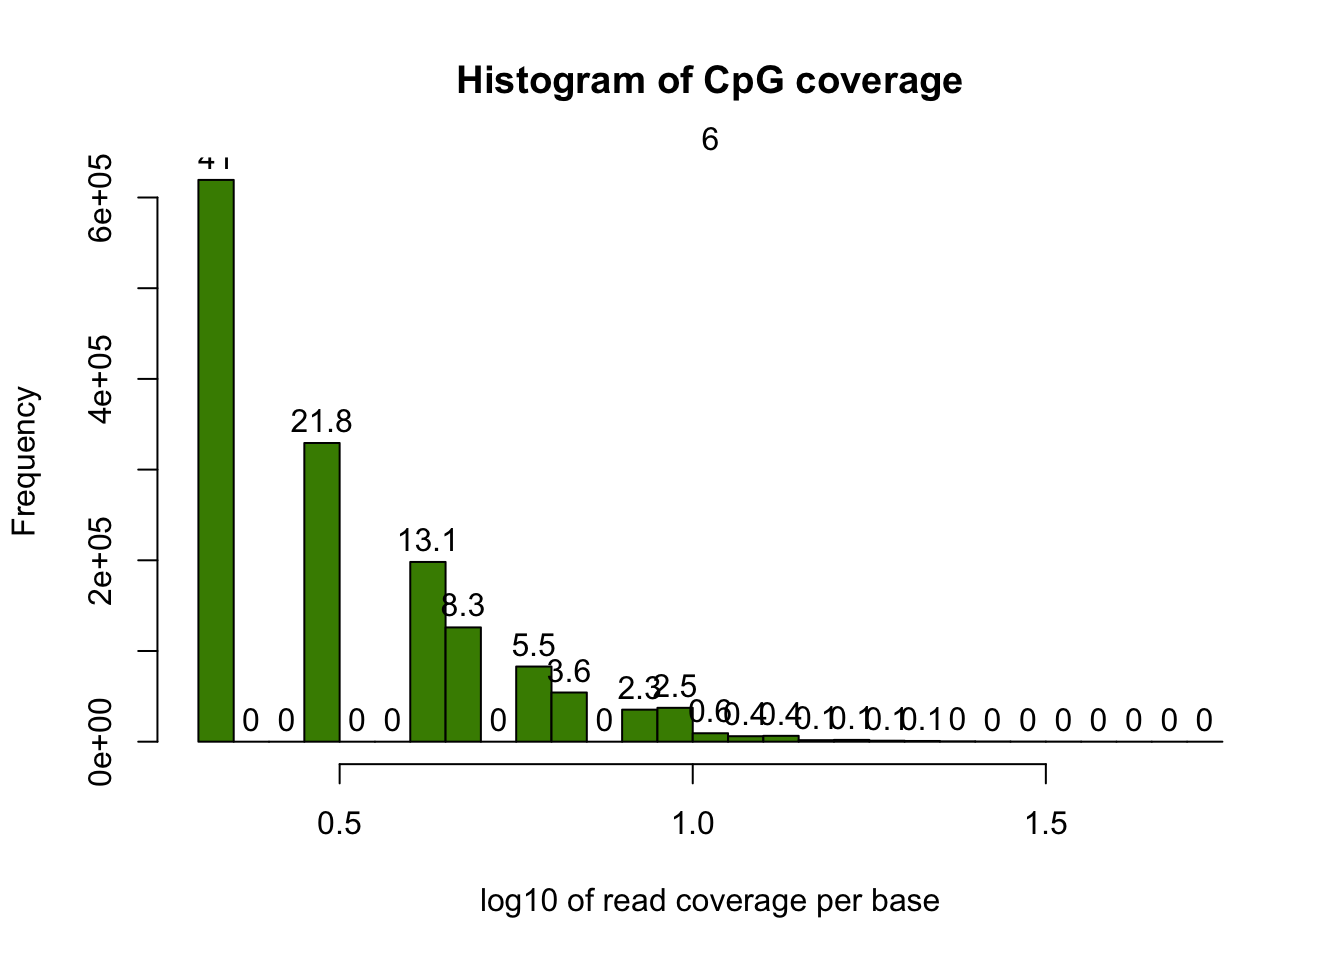
\includegraphics{02-matrices_files/figure-latex/unnamed-chunk-5-6.pdf}
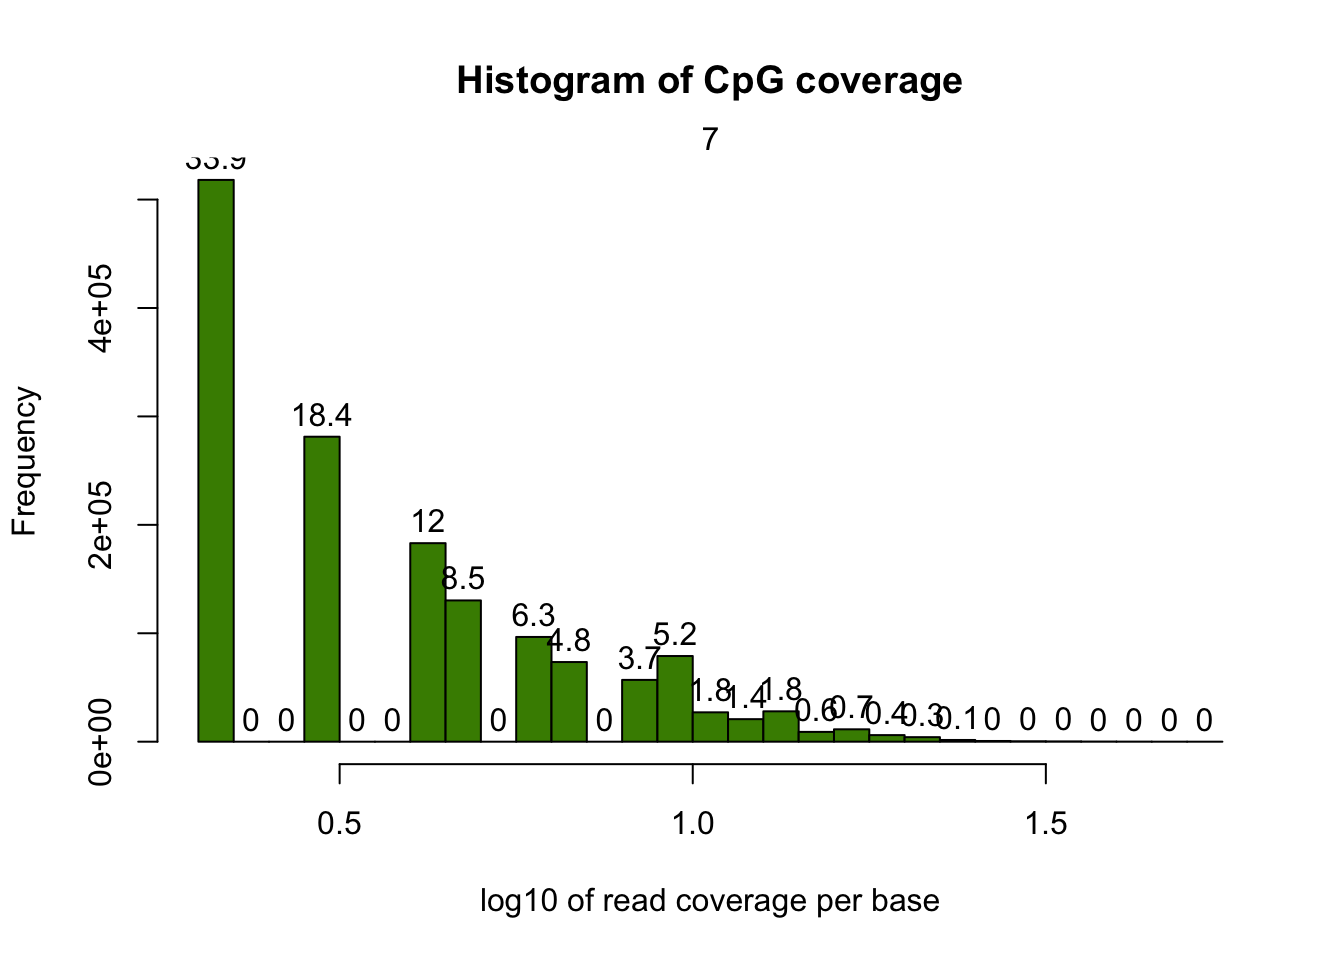
\includegraphics{02-matrices_files/figure-latex/unnamed-chunk-5-7.pdf}
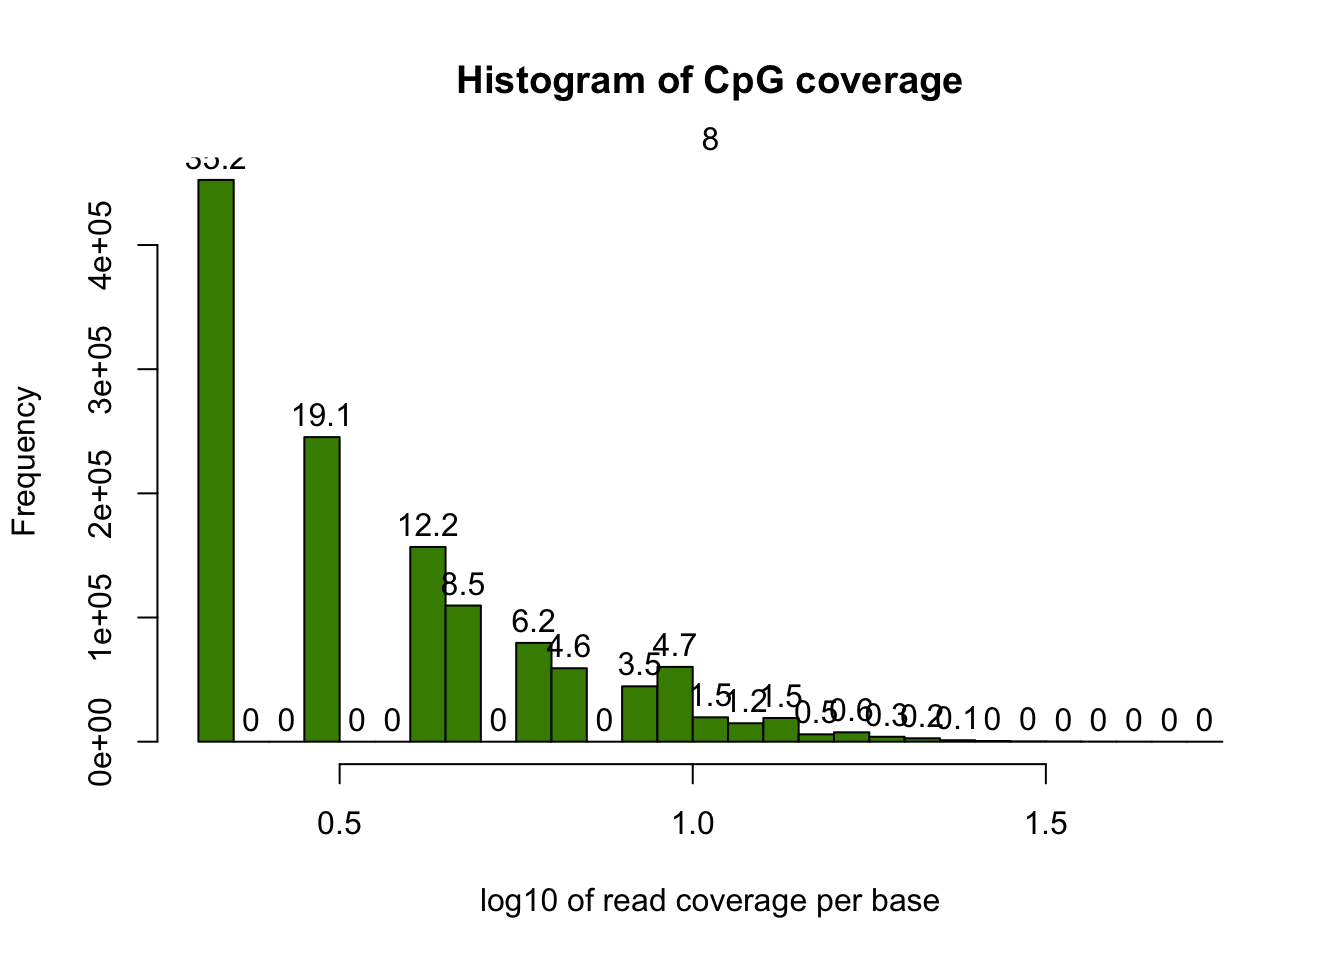
\includegraphics{02-matrices_files/figure-latex/unnamed-chunk-5-8.pdf}
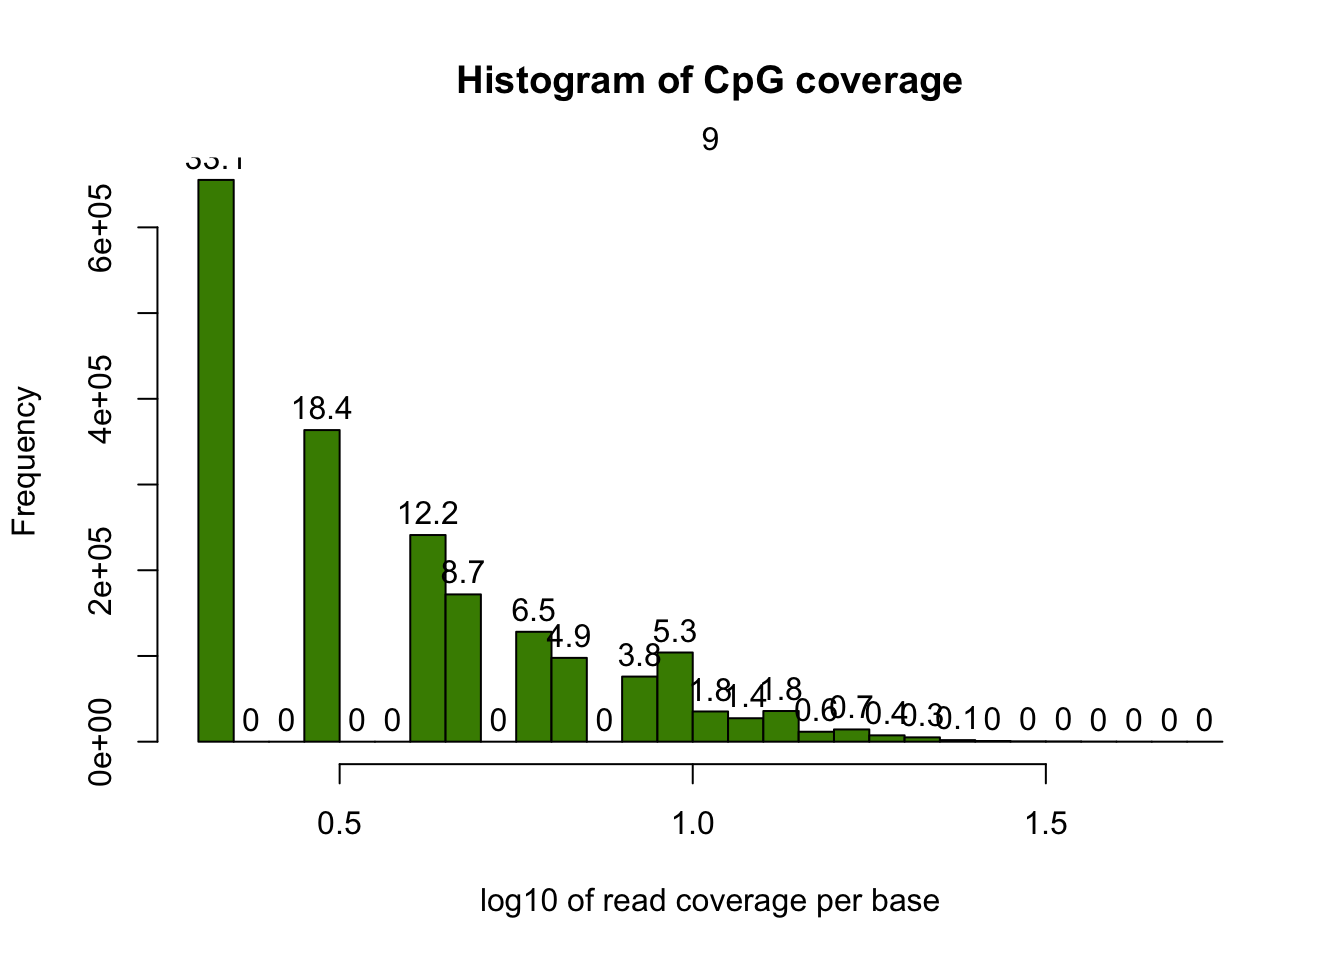
\includegraphics{02-matrices_files/figure-latex/unnamed-chunk-5-9.pdf}
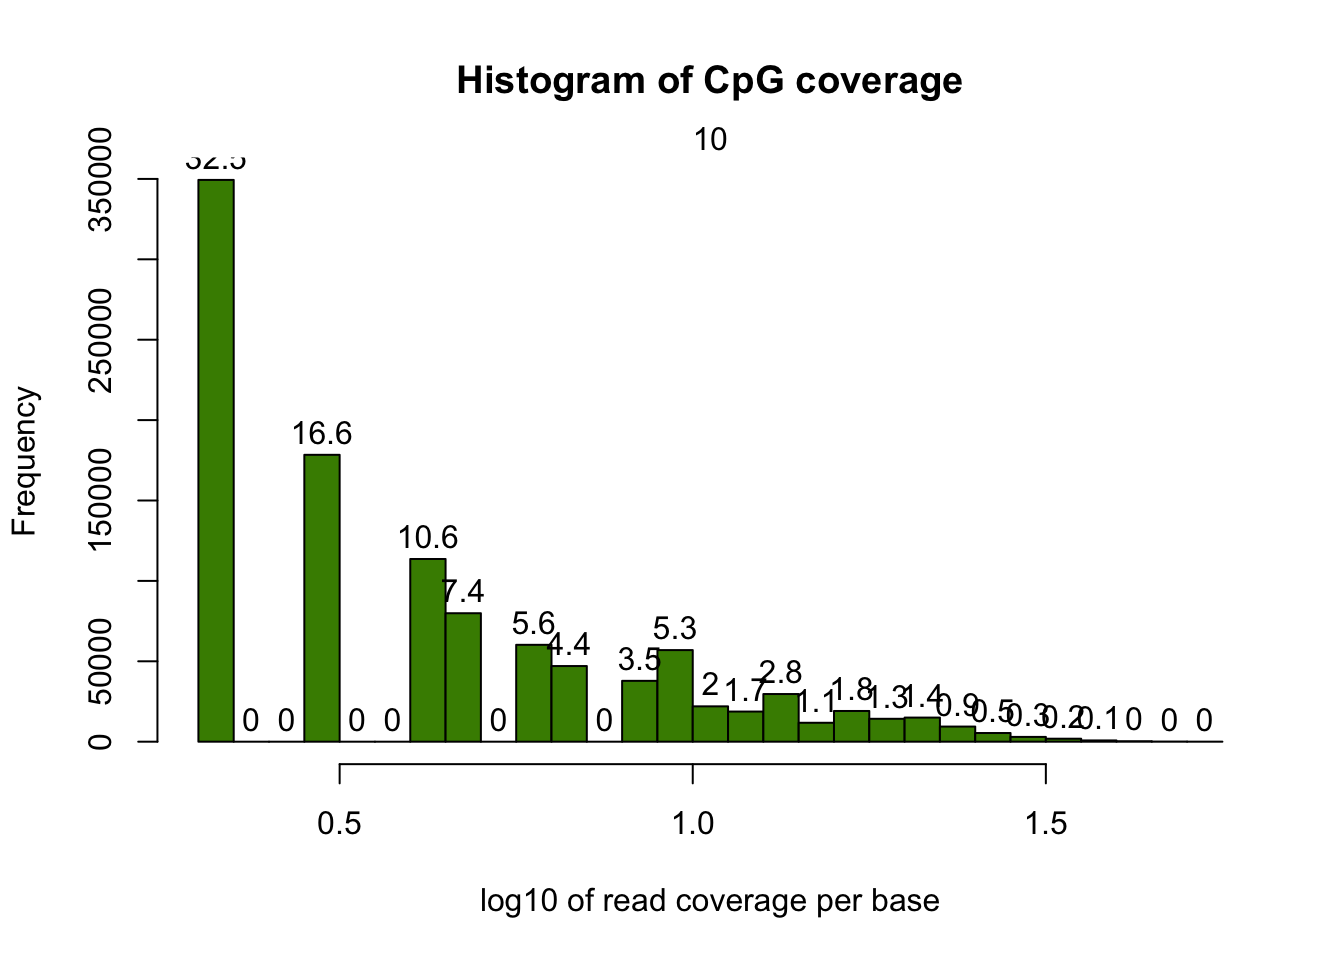
\includegraphics{02-matrices_files/figure-latex/unnamed-chunk-5-10.pdf}
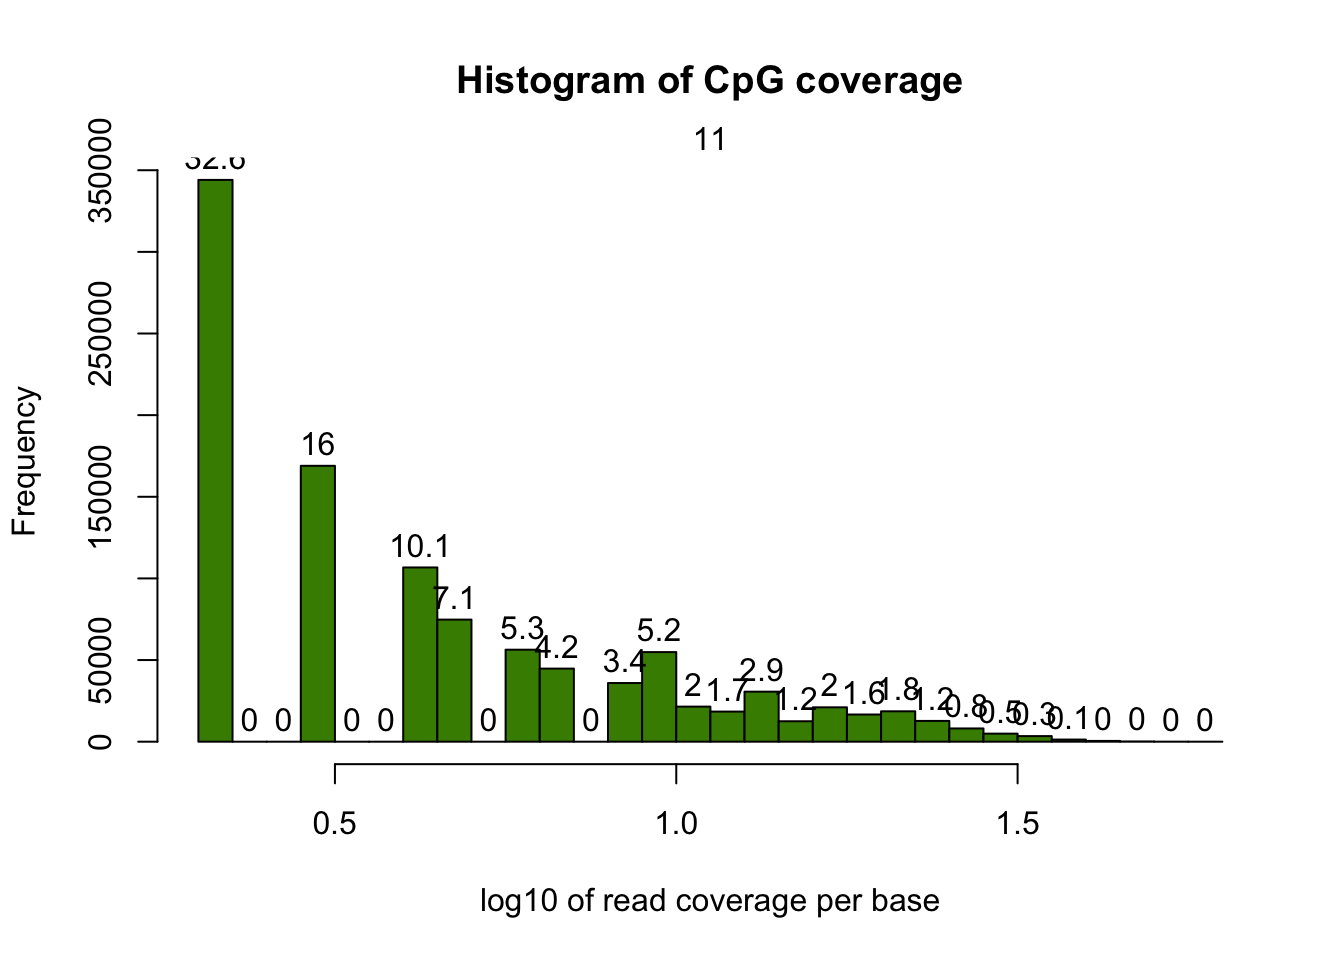
\includegraphics{02-matrices_files/figure-latex/unnamed-chunk-5-11.pdf}
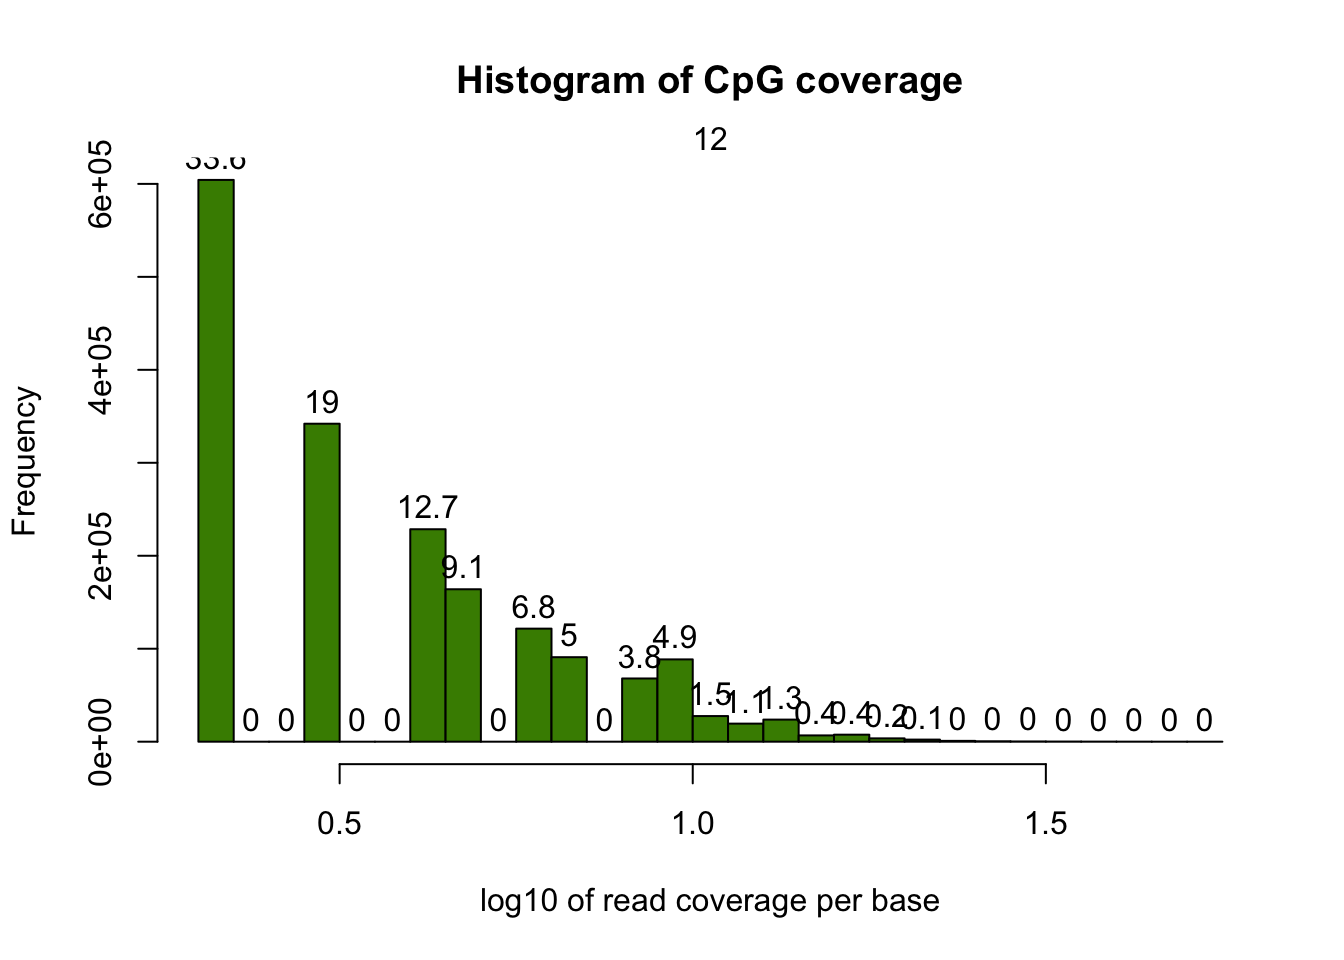
\includegraphics{02-matrices_files/figure-latex/unnamed-chunk-5-12.pdf}
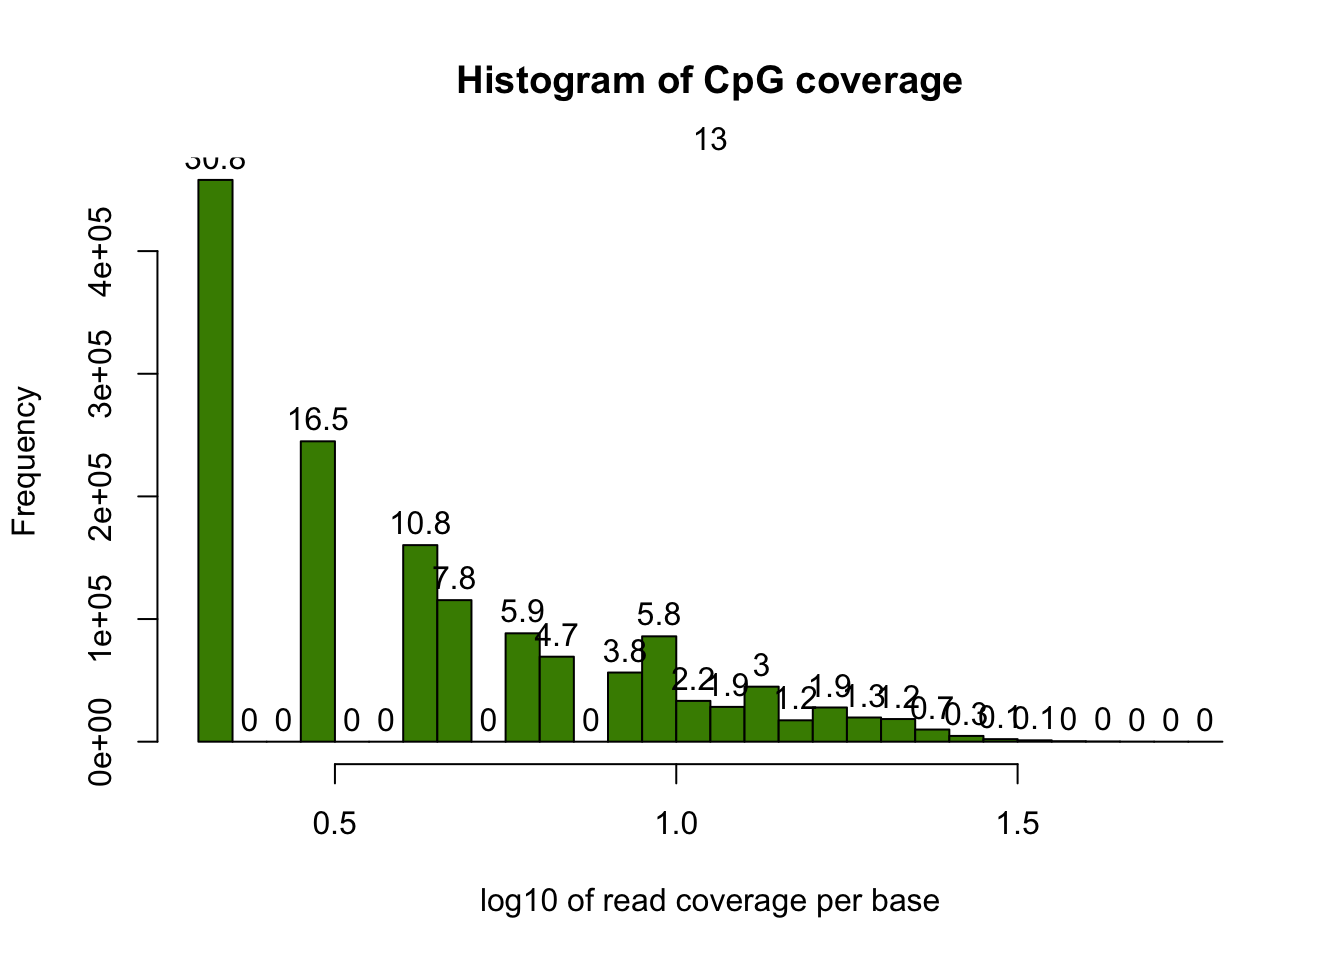
\includegraphics{02-matrices_files/figure-latex/unnamed-chunk-5-13.pdf}
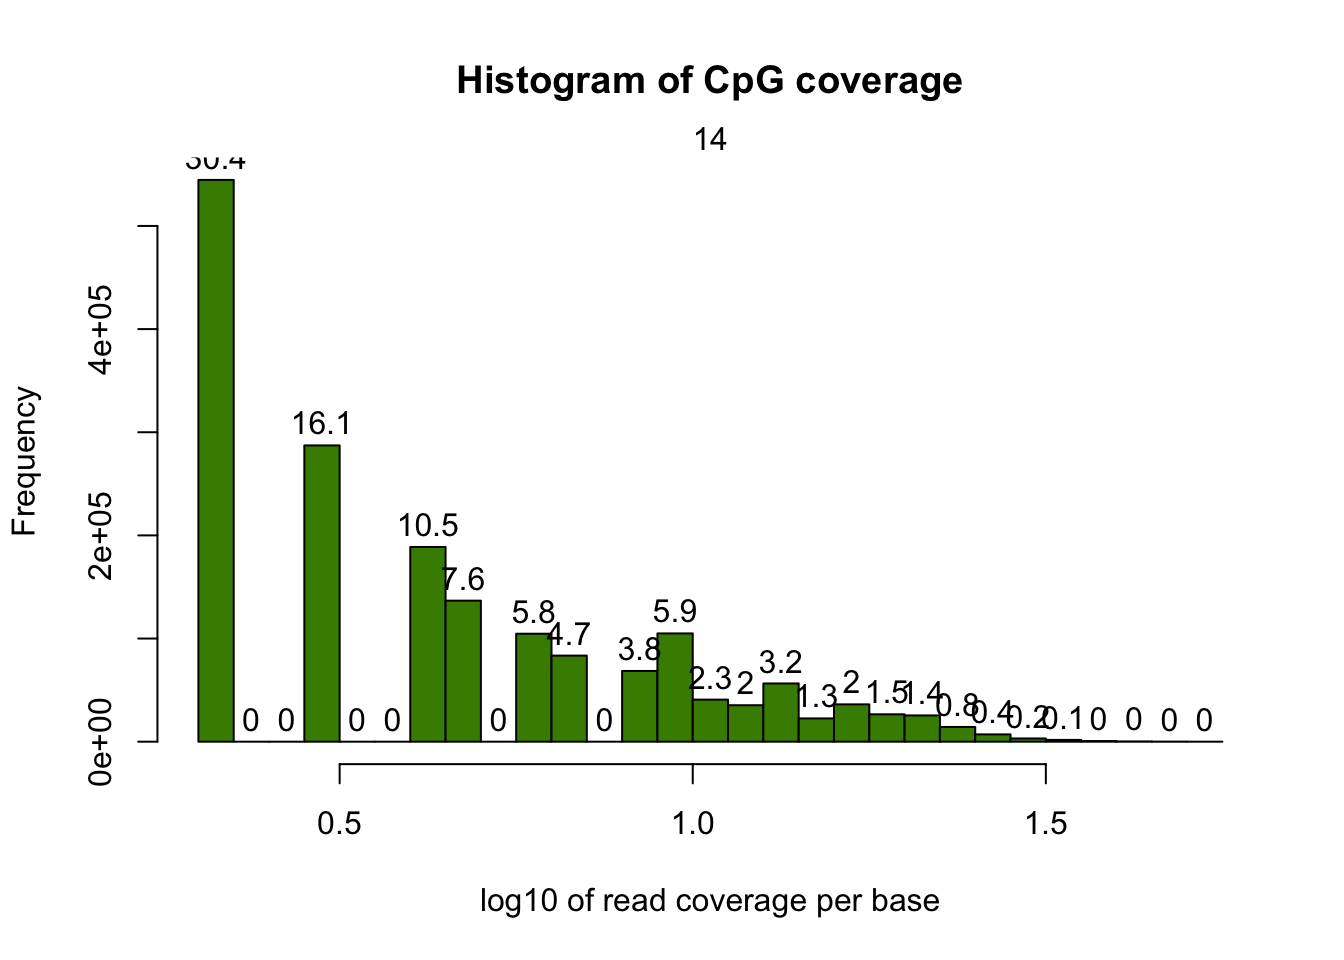
\includegraphics{02-matrices_files/figure-latex/unnamed-chunk-5-14.pdf}
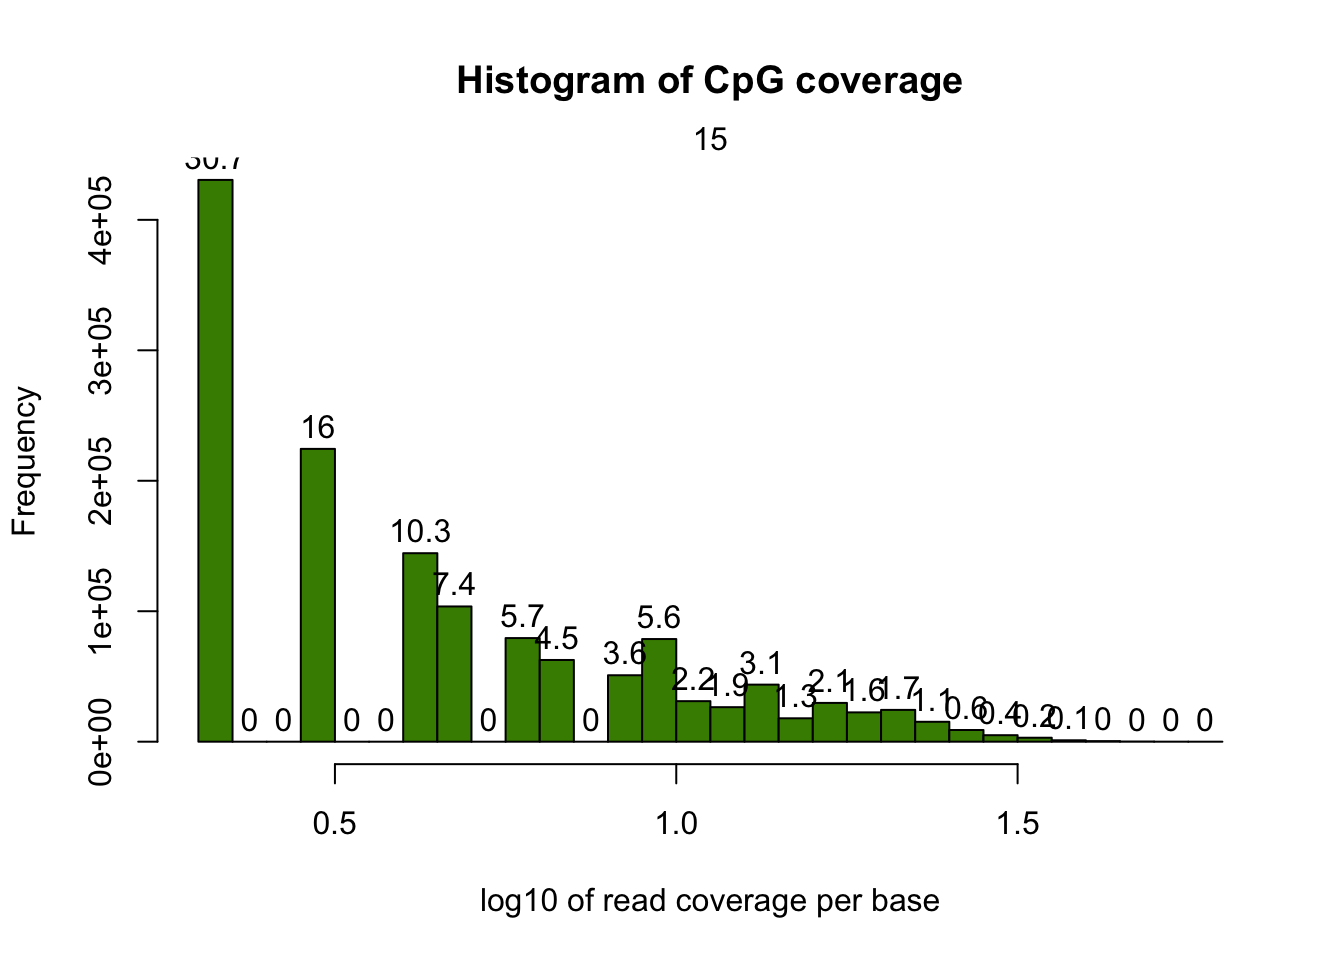
\includegraphics{02-matrices_files/figure-latex/unnamed-chunk-5-15.pdf}
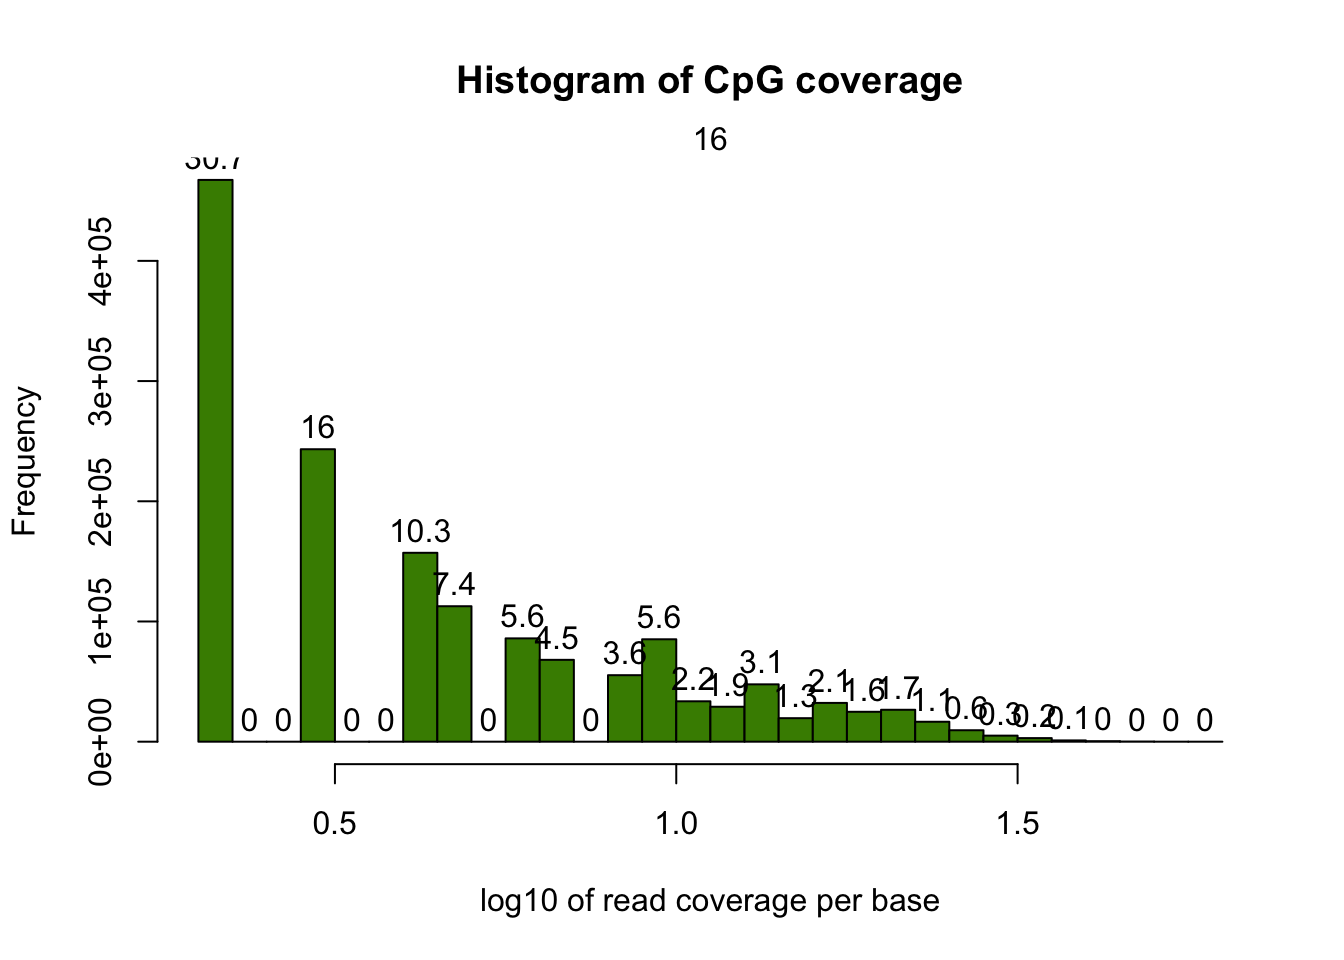
\includegraphics{02-matrices_files/figure-latex/unnamed-chunk-5-16.pdf}
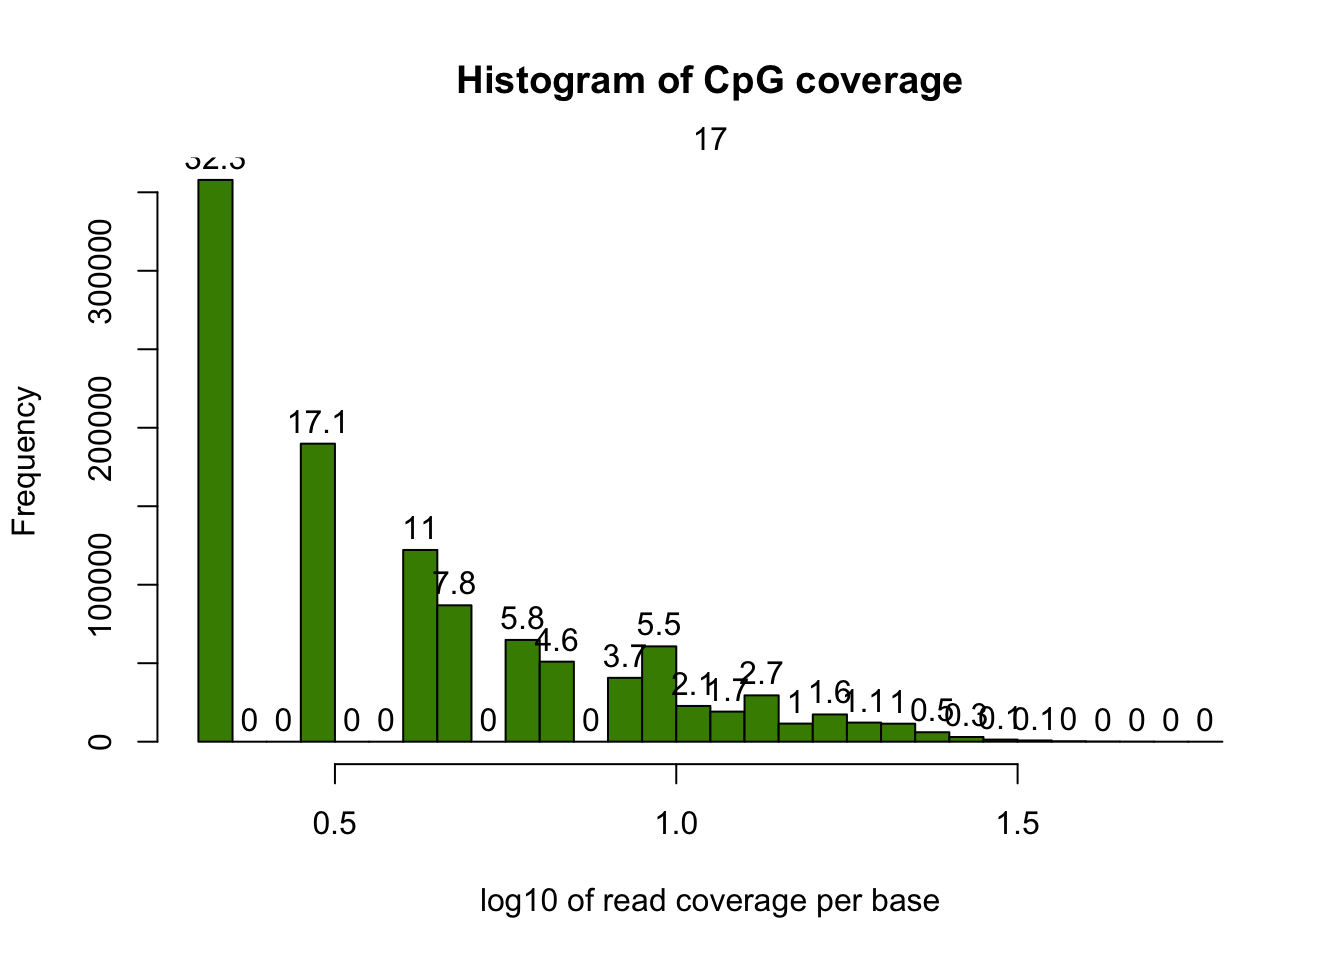
\includegraphics{02-matrices_files/figure-latex/unnamed-chunk-5-17.pdf}
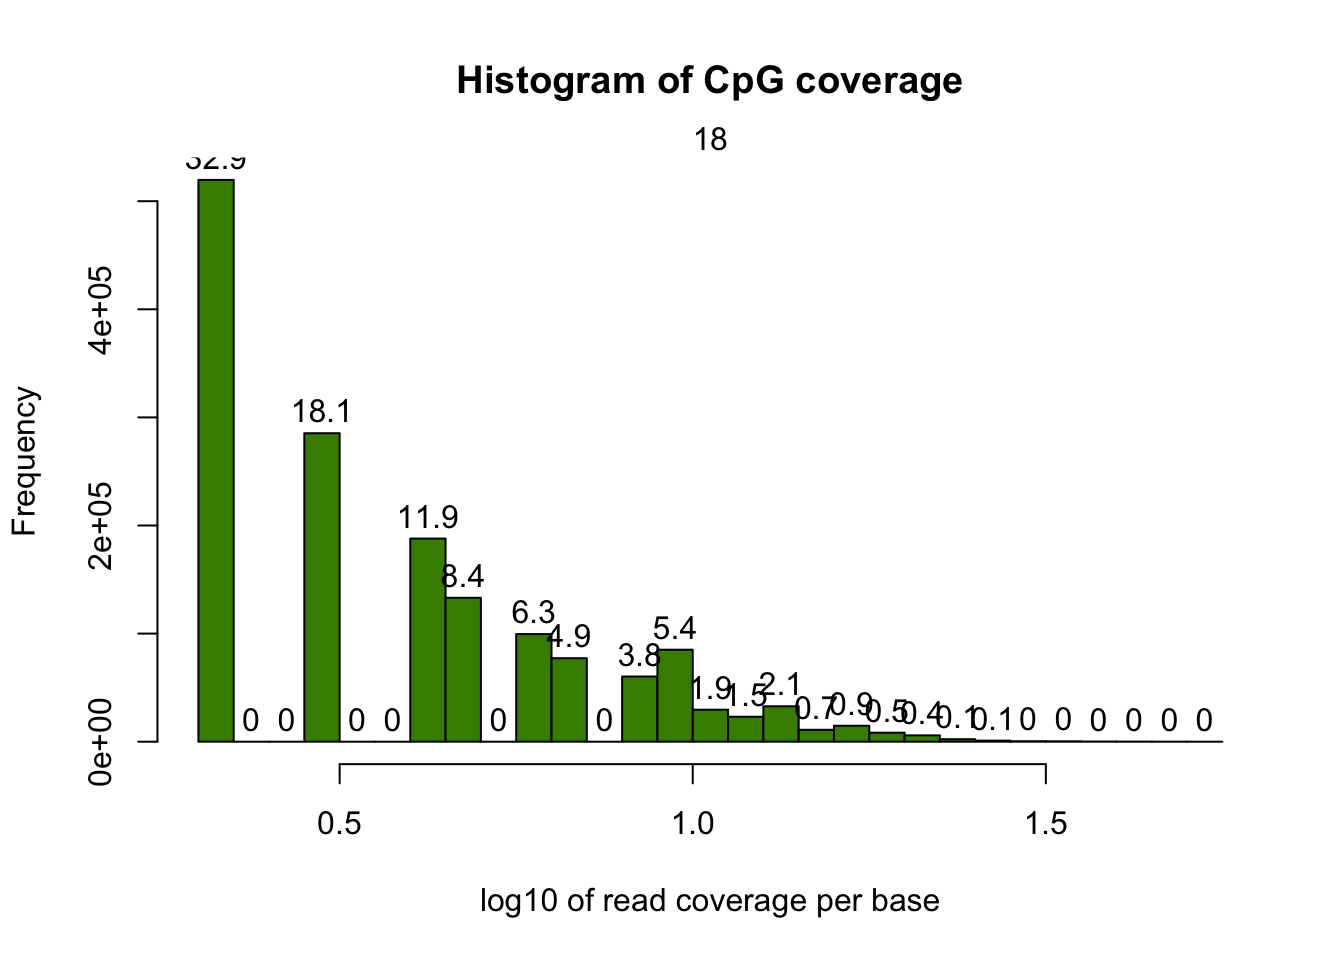
\includegraphics{02-matrices_files/figure-latex/unnamed-chunk-5-18.pdf}

It might be useful to filter samples based on coverage. Particularly, if
our samples are suffering from PCR bias it would be useful to discard
bases with very high read coverage. Furthermore, we would also like to
discard bases that have low read coverage, a high enough read coverage
will increase the power of the statistical tests. The code below creates
two objects by filtering the methylRawList and discards bases that have
coverage below 10X, and below 5x (but no max coverage is set b/c/
hi.perc=100. Could consider discarding the bases that have more than
99.9th percentile of coverage in each sample.)

\begin{Shaded}
\begin{Highlighting}[]
\NormalTok{filtered10.myobj=}\KeywordTok{filterByCoverage}\NormalTok{(myobj_}\DecValTok{18}\NormalTok{,}\DataTypeTok{lo.count=}\DecValTok{10}\NormalTok{,}\DataTypeTok{lo.perc=}\OtherTok{NULL}\NormalTok{,}
                                      \DataTypeTok{hi.count=}\DecValTok{100}\NormalTok{,}\DataTypeTok{hi.perc=}\OtherTok{NULL}\NormalTok{)}

\NormalTok{filtered5.myobj=}\KeywordTok{filterByCoverage}\NormalTok{(myobj_}\DecValTok{18}\NormalTok{,}\DataTypeTok{lo.count=}\DecValTok{5}\NormalTok{,}\DataTypeTok{lo.perc=}\OtherTok{NULL}\NormalTok{,}
                                      \DataTypeTok{hi.count=}\DecValTok{100}\NormalTok{,}\DataTypeTok{hi.perc=}\OtherTok{NULL}\NormalTok{)}
\end{Highlighting}
\end{Shaded}

In order to do further analysis, we will need to get the bases covered
in all samples. The following function will merge all samples to one
object for base-pair locations that are covered in all samples. Setting
destrand=TRUE (the default is FALSE) will merge reads on both strands of
a CpG dinucleotide. This provides better coverage, but only advised when
looking at CpG methylation (for CpH methylation this will cause wrong
results in subsequent analyses). In addition, setting destrand=TRUE will
only work when operating on base-pair resolution, otherwise setting this
option TRUE will have no effect. The unite() function will return a
methylBase object which will be our main object for all comparative
analysis. The methylBase object contains methylation information for
regions/bases that are covered in all samples.

By default, unite function produces bases/regions covered in all
samples. That requirement can be relaxed using ``min.per.group'' option
in unite function. For example, to create a methylBase object where only
CpGs covered with at least 1 sample per group (i.e.~treatment, defined
upon reading in Bismark alignment file) will be returned:
\texttt{meth.min=unite(myobj,min.per.group=1L)}

In this case, we use the default which is to require coverage across all
samples. Also, we create 2 methylBase objects: coverage
\textgreater{}=10x, and coverage \textgreater{}=5x

\begin{Shaded}
\begin{Highlighting}[]
\NormalTok{meth_filter10=}\KeywordTok{unite}\NormalTok{(filtered10.myobj, }\DataTypeTok{destrand=}\OtherTok{TRUE}\NormalTok{)}
\NormalTok{meth_filter5=}\KeywordTok{unite}\NormalTok{(filtered5.myobj, }\DataTypeTok{destrand=}\OtherTok{TRUE}\NormalTok{)}
\end{Highlighting}
\end{Shaded}

We can check the correlation (default=Pearson) between samples using
getCorrelation. This function will either plot scatter plot and
correlation coefficients or just print a correlation matrix. (I'm
showing w/o plotting; takes too much time)

\begin{Shaded}
\begin{Highlighting}[]
\KeywordTok{getCorrelation}\NormalTok{(meth_filter10,}\DataTypeTok{plot=}\OtherTok{FALSE}\NormalTok{) }\CommentTok{#correlation matrix, 10x coverage}
\end{Highlighting}
\end{Shaded}

\begin{verbatim}
##            1         2         3         4         5         6         7
## 1  1.0000000 0.6474827 0.6666848 0.6762287 0.6392971 0.7017533 0.6541630
## 2  0.6474827 1.0000000 0.6800761 0.7053758 0.6570977 0.6345348 0.6716664
## 3  0.6666848 0.6800761 1.0000000 0.7151097 0.6663944 0.6442118 0.7302352
## 4  0.6762287 0.7053758 0.7151097 1.0000000 0.6602668 0.6587420 0.7051690
## 5  0.6392971 0.6570977 0.6663944 0.6602668 1.0000000 0.6326074 0.7128529
## 6  0.7017533 0.6345348 0.6442118 0.6587420 0.6326074 1.0000000 0.6221249
## 7  0.6541630 0.6716664 0.7302352 0.7051690 0.7128529 0.6221249 1.0000000
## 8  0.6820820 0.6466106 0.6528931 0.6701398 0.6183613 0.6793876 0.6345836
## 9  0.6473843 0.6400475 0.6647439 0.6472976 0.6463275 0.6175413 0.6511168
## 10 0.6532630 0.6483994 0.6618212 0.6665623 0.6579780 0.6329433 0.6705518
## 11 0.6253457 0.6196995 0.6440825 0.6519309 0.6281219 0.6067272 0.6447527
## 12 0.6300573 0.6315207 0.6250652 0.6247597 0.6524651 0.6132448 0.6179600
## 13 0.6582075 0.6595815 0.6690174 0.6605324 0.6575865 0.6471854 0.6610663
## 14 0.6591828 0.6448005 0.6657464 0.6578911 0.6430044 0.6347740 0.6555664
## 15 0.6434660 0.6474434 0.6648987 0.6678681 0.6271321 0.6268320 0.6715743
## 16 0.6619737 0.6517417 0.6542004 0.6521972 0.6514878 0.6253665 0.6544498
## 17 0.6509435 0.6494889 0.6538636 0.6569427 0.6445617 0.6374211 0.6532621
## 18 0.6599287 0.6569770 0.6667105 0.6592379 0.6670609 0.6401146 0.6605606
##            8         9        10        11        12        13        14
## 1  0.6820820 0.6473843 0.6532630 0.6253457 0.6300573 0.6582075 0.6591828
## 2  0.6466106 0.6400475 0.6483994 0.6196995 0.6315207 0.6595815 0.6448005
## 3  0.6528931 0.6647439 0.6618212 0.6440825 0.6250652 0.6690174 0.6657464
## 4  0.6701398 0.6472976 0.6665623 0.6519309 0.6247597 0.6605324 0.6578911
## 5  0.6183613 0.6463275 0.6579780 0.6281219 0.6524651 0.6575865 0.6430044
## 6  0.6793876 0.6175413 0.6329433 0.6067272 0.6132448 0.6471854 0.6347740
## 7  0.6345836 0.6511168 0.6705518 0.6447527 0.6179600 0.6610663 0.6555664
## 8  1.0000000 0.6172210 0.6218287 0.6107849 0.6028061 0.6419895 0.6435372
## 9  0.6172210 1.0000000 0.6528998 0.6222314 0.6280387 0.6537493 0.6546545
## 10 0.6218287 0.6528998 1.0000000 0.7213455 0.6938524 0.7325784 0.7147908
## 11 0.6107849 0.6222314 0.7213455 1.0000000 0.6514273 0.7242441 0.7053775
## 12 0.6028061 0.6280387 0.6938524 0.6514273 1.0000000 0.7190977 0.6804995
## 13 0.6419895 0.6537493 0.7325784 0.7242441 0.7190977 1.0000000 0.7316778
## 14 0.6435372 0.6546545 0.7147908 0.7053775 0.6804995 0.7316778 1.0000000
## 15 0.6355816 0.6199579 0.6802428 0.6789533 0.6280124 0.6837751 0.6827601
## 16 0.6271593 0.6392529 0.7161549 0.7154545 0.6646392 0.7421678 0.7437519
## 17 0.6690379 0.6383191 0.6925906 0.6609847 0.6457725 0.6842226 0.6784860
## 18 0.6367324 0.6486887 0.7138594 0.6949911 0.7104654 0.7641980 0.7360778
##           15        16        17        18
## 1  0.6434660 0.6619737 0.6509435 0.6599287
## 2  0.6474434 0.6517417 0.6494889 0.6569770
## 3  0.6648987 0.6542004 0.6538636 0.6667105
## 4  0.6678681 0.6521972 0.6569427 0.6592379
## 5  0.6271321 0.6514878 0.6445617 0.6670609
## 6  0.6268320 0.6253665 0.6374211 0.6401146
## 7  0.6715743 0.6544498 0.6532621 0.6605606
## 8  0.6355816 0.6271593 0.6690379 0.6367324
## 9  0.6199579 0.6392529 0.6383191 0.6486887
## 10 0.6802428 0.7161549 0.6925906 0.7138594
## 11 0.6789533 0.7154545 0.6609847 0.6949911
## 12 0.6280124 0.6646392 0.6457725 0.7104654
## 13 0.6837751 0.7421678 0.6842226 0.7641980
## 14 0.6827601 0.7437519 0.6784860 0.7360778
## 15 1.0000000 0.6837052 0.6635478 0.6530284
## 16 0.6837052 1.0000000 0.6856313 0.7071251
## 17 0.6635478 0.6856313 1.0000000 0.6825180
## 18 0.6530284 0.7071251 0.6825180 1.0000000
\end{verbatim}

\begin{Shaded}
\begin{Highlighting}[]
\KeywordTok{getCorrelation}\NormalTok{(meth_filter5,}\DataTypeTok{plot=}\OtherTok{FALSE}\NormalTok{)  }\CommentTok{#correlation matrix, 5x coverage}
\end{Highlighting}
\end{Shaded}

\begin{verbatim}
##            1         2         3         4         5         6         7
## 1  1.0000000 0.5203324 0.5282404 0.5277955 0.5022175 0.5899275 0.5270635
## 2  0.5203324 1.0000000 0.5589683 0.5914152 0.5341853 0.4954366 0.5759710
## 3  0.5282404 0.5589683 1.0000000 0.5906174 0.5438585 0.4999331 0.6128457
## 4  0.5277955 0.5914152 0.5906174 1.0000000 0.5232693 0.5060093 0.5862341
## 5  0.5022175 0.5341853 0.5438585 0.5232693 1.0000000 0.4852987 0.6087552
## 6  0.5899275 0.4954366 0.4999331 0.5060093 0.4852987 1.0000000 0.4903991
## 7  0.5270635 0.5759710 0.6128457 0.5862341 0.6087552 0.4903991 1.0000000
## 8  0.5715679 0.5176748 0.5164720 0.5317901 0.4933246 0.5579952 0.5107628
## 9  0.5302612 0.5317613 0.5352212 0.5247550 0.5151886 0.5025897 0.5288700
## 10 0.5278785 0.5134400 0.5230536 0.5257591 0.5040114 0.5017013 0.5304511
## 11 0.5148343 0.5012486 0.5179590 0.5152580 0.4876532 0.4854534 0.5200991
## 12 0.5054842 0.5073348 0.4942885 0.4958185 0.5077958 0.4901367 0.5000016
## 13 0.5513353 0.5347206 0.5499918 0.5495005 0.5202891 0.5164031 0.5558191
## 14 0.5477871 0.5303936 0.5488113 0.5432307 0.5190625 0.5168156 0.5493498
## 15 0.5349181 0.5160514 0.5289485 0.5418185 0.5065675 0.5084176 0.5309964
## 16 0.5398558 0.5198102 0.5376549 0.5354271 0.5108783 0.5010364 0.5408960
## 17 0.5334805 0.5227479 0.5262968 0.5345332 0.5021054 0.5064655 0.5215438
## 18 0.5297419 0.5291267 0.5375875 0.5319430 0.5223619 0.5088418 0.5348182
##            8         9        10        11        12        13        14
## 1  0.5715679 0.5302612 0.5278785 0.5148343 0.5054842 0.5513353 0.5477871
## 2  0.5176748 0.5317613 0.5134400 0.5012486 0.5073348 0.5347206 0.5303936
## 3  0.5164720 0.5352212 0.5230536 0.5179590 0.4942885 0.5499918 0.5488113
## 4  0.5317901 0.5247550 0.5257591 0.5152580 0.4958185 0.5495005 0.5432307
## 5  0.4933246 0.5151886 0.5040114 0.4876532 0.5077958 0.5202891 0.5190625
## 6  0.5579952 0.5025897 0.5017013 0.4854534 0.4901367 0.5164031 0.5168156
## 7  0.5107628 0.5288700 0.5304511 0.5200991 0.5000016 0.5558191 0.5493498
## 8  1.0000000 0.5123594 0.5097867 0.5048310 0.4844548 0.5262421 0.5302390
## 9  0.5123594 1.0000000 0.5365803 0.5173040 0.5248426 0.5529726 0.5488203
## 10 0.5097867 0.5365803 1.0000000 0.6216062 0.5828120 0.6515680 0.6316178
## 11 0.5048310 0.5173040 0.6216062 1.0000000 0.5355448 0.6369405 0.6098844
## 12 0.4844548 0.5248426 0.5828120 0.5355448 1.0000000 0.6250909 0.5949646
## 13 0.5262421 0.5529726 0.6515680 0.6369405 0.6250909 1.0000000 0.6630315
## 14 0.5302390 0.5488203 0.6316178 0.6098844 0.5949646 0.6630315 1.0000000
## 15 0.5285563 0.5288093 0.5607748 0.5503544 0.5095783 0.5853971 0.5788881
## 16 0.5182491 0.5428453 0.6283167 0.6233602 0.5583828 0.6595183 0.6573833
## 17 0.5292731 0.5383151 0.5647206 0.5511178 0.5263066 0.5815727 0.5732395
## 18 0.5146142 0.5439974 0.5990934 0.5769738 0.6198649 0.6810999 0.6498659
##           15        16        17        18
## 1  0.5349181 0.5398558 0.5334805 0.5297419
## 2  0.5160514 0.5198102 0.5227479 0.5291267
## 3  0.5289485 0.5376549 0.5262968 0.5375875
## 4  0.5418185 0.5354271 0.5345332 0.5319430
## 5  0.5065675 0.5108783 0.5021054 0.5223619
## 6  0.5084176 0.5010364 0.5064655 0.5088418
## 7  0.5309964 0.5408960 0.5215438 0.5348182
## 8  0.5285563 0.5182491 0.5292731 0.5146142
## 9  0.5288093 0.5428453 0.5383151 0.5439974
## 10 0.5607748 0.6283167 0.5647206 0.5990934
## 11 0.5503544 0.6233602 0.5511178 0.5769738
## 12 0.5095783 0.5583828 0.5263066 0.6198649
## 13 0.5853971 0.6595183 0.5815727 0.6810999
## 14 0.5788881 0.6573833 0.5732395 0.6498659
## 15 1.0000000 0.5760357 0.5620237 0.5574024
## 16 0.5760357 1.0000000 0.5793753 0.6167757
## 17 0.5620237 0.5793753 1.0000000 0.5624481
## 18 0.5574024 0.6167757 0.5624481 1.0000000
\end{verbatim}

We can cluster the samples based on the similarity of their methylation
profiles. The following function will cluster the samples and draw a
dendrogram.

\begin{Shaded}
\begin{Highlighting}[]
\KeywordTok{clusterSamples}\NormalTok{(meth_filter10, }\DataTypeTok{dist=}\StringTok{"correlation"}\NormalTok{, }\DataTypeTok{method=}\StringTok{"ward"}\NormalTok{, }\DataTypeTok{plot=}\OtherTok{TRUE}\NormalTok{) }\CommentTok{#cluster analysis 10x, correlation matrix}
\end{Highlighting}
\end{Shaded}

\begin{verbatim}
## The "ward" method has been renamed to "ward.D"; note new "ward.D2"
\end{verbatim}

\includegraphics{02-matrices_files/figure-latex/unnamed-chunk-9-1.pdf}

\begin{verbatim}
## 
## Call:
## hclust(d = d, method = HCLUST.METHODS[hclust.method])
## 
## Cluster method   : ward.D 
## Distance         : pearson 
## Number of objects: 18
\end{verbatim}

\begin{Shaded}
\begin{Highlighting}[]
\KeywordTok{clusterSamples}\NormalTok{(meth_filter5, }\DataTypeTok{dist=}\StringTok{"correlation"}\NormalTok{, }\DataTypeTok{method=}\StringTok{"ward"}\NormalTok{, }\DataTypeTok{plot=}\OtherTok{TRUE}\NormalTok{) }\CommentTok{#cluster analysis 5x, correlation matrix}
\end{Highlighting}
\end{Shaded}

\begin{verbatim}
## The "ward" method has been renamed to "ward.D"; note new "ward.D2"
\end{verbatim}

\includegraphics{02-matrices_files/figure-latex/unnamed-chunk-9-2.pdf}

\begin{verbatim}
## 
## Call:
## hclust(d = d, method = HCLUST.METHODS[hclust.method])
## 
## Cluster method   : ward.D 
## Distance         : pearson 
## Number of objects: 18
\end{verbatim}

\begin{Shaded}
\begin{Highlighting}[]
\KeywordTok{clusterSamples}\NormalTok{(meth_filter10, }\DataTypeTok{dist=}\StringTok{"manhattan"}\NormalTok{, }\DataTypeTok{method=}\StringTok{"ward"}\NormalTok{, }\DataTypeTok{plot=}\OtherTok{TRUE}\NormalTok{)  }\CommentTok{#cluster analysis 10x, manhattan distance matrix}
\end{Highlighting}
\end{Shaded}

\begin{verbatim}
## The "ward" method has been renamed to "ward.D"; note new "ward.D2"
\end{verbatim}

\includegraphics{02-matrices_files/figure-latex/unnamed-chunk-9-3.pdf}

\begin{verbatim}
## 
## Call:
## hclust(d = d, method = HCLUST.METHODS[hclust.method])
## 
## Cluster method   : ward.D 
## Distance         : manhattan 
## Number of objects: 18
\end{verbatim}

\begin{Shaded}
\begin{Highlighting}[]
\KeywordTok{clusterSamples}\NormalTok{(meth_filter5, }\DataTypeTok{dist=}\StringTok{"manhattan"}\NormalTok{, }\DataTypeTok{method=}\StringTok{"ward"}\NormalTok{, }\DataTypeTok{plot=}\OtherTok{TRUE}\NormalTok{)  }\CommentTok{#cluster analysis 5x, manhattan distance matrix}
\end{Highlighting}
\end{Shaded}

\begin{verbatim}
## The "ward" method has been renamed to "ward.D"; note new "ward.D2"
\end{verbatim}

\includegraphics{02-matrices_files/figure-latex/unnamed-chunk-9-4.pdf}

\begin{verbatim}
## 
## Call:
## hclust(d = d, method = HCLUST.METHODS[hclust.method])
## 
## Cluster method   : ward.D 
## Distance         : manhattan 
## Number of objects: 18
\end{verbatim}

\begin{Shaded}
\begin{Highlighting}[]
\KeywordTok{PCASamples}\NormalTok{(meth_filter10)}
\end{Highlighting}
\end{Shaded}

\includegraphics{02-matrices_files/figure-latex/unnamed-chunk-10-1.pdf}

\begin{Shaded}
\begin{Highlighting}[]
\KeywordTok{PCASamples}\NormalTok{(meth_filter5)}
\end{Highlighting}
\end{Shaded}

\includegraphics{02-matrices_files/figure-latex/unnamed-chunk-10-2.pdf}

Percent methylation matrix (rows=region/base, columns=sample) can be
extracted from methylBase object by using percMethylation function. This
can be useful for downstream analyses.

\begin{Shaded}
\begin{Highlighting}[]
\NormalTok{perc.meth10=}\KeywordTok{percMethylation}\NormalTok{(meth_filter10, }\DataTypeTok{rowids=}\NormalTok{T)}
\NormalTok{perc.meth5=}\KeywordTok{percMethylation}\NormalTok{(meth_filter5, }\DataTypeTok{rowids=}\NormalTok{T)}
\end{Highlighting}
\end{Shaded}

Extract correlation matrix (pearson) and distance matrix (manhattan)
from the \% methylated matrix FYI I checked that the correlation matrix
in \texttt{getCorrelation} is derived from the percent methylated
matrix. It is!

\begin{Shaded}
\begin{Highlighting}[]
\NormalTok{cor.pears.}\DecValTok{10}\NormalTok{ <-}\StringTok{ }\KeywordTok{cor}\NormalTok{(perc.meth10, }\DataTypeTok{method=}\StringTok{"pearson"}\NormalTok{) }\CommentTok{# create pearson correlation matrix. }
\NormalTok{dist.manhat.}\DecValTok{10}\NormalTok{ <-}\StringTok{ }\KeywordTok{dist}\NormalTok{(}\KeywordTok{t}\NormalTok{(perc.meth10), }\DataTypeTok{method =} \StringTok{"manhattan"}\NormalTok{, }\DataTypeTok{diag =}\NormalTok{ T, }\DataTypeTok{upper =}\NormalTok{ F)}
\NormalTok{dist.manhat.}\FloatTok{10.}\NormalTok{df <-}\StringTok{ }\NormalTok{reshape2}\OperatorTok{::}\KeywordTok{melt}\NormalTok{(}\KeywordTok{as.matrix}\NormalTok{(dist.manhat.}\DecValTok{10}\NormalTok{), }\DataTypeTok{varnames =} \KeywordTok{c}\NormalTok{(}\StringTok{"row"}\NormalTok{, }\StringTok{"col"}\NormalTok{))}

\NormalTok{cor.pears.}\DecValTok{5}\NormalTok{ <-}\StringTok{ }\KeywordTok{cor}\NormalTok{(perc.meth5, }\DataTypeTok{method=}\StringTok{"pearson"}\NormalTok{) }\CommentTok{# create pearson correlation matrix. }
\NormalTok{dist.manhat.}\DecValTok{5}\NormalTok{ <-}\StringTok{ }\KeywordTok{dist}\NormalTok{(}\KeywordTok{t}\NormalTok{(perc.meth5), }\DataTypeTok{method =} \StringTok{"manhattan"}\NormalTok{, }\DataTypeTok{diag =}\NormalTok{ T, }\DataTypeTok{upper =}\NormalTok{ F) }\CommentTok{#must transform % matrix (samples are rows) for the dist() function}
\NormalTok{dist.manhat.}\FloatTok{5.}\NormalTok{df <-}\StringTok{ }\NormalTok{reshape2}\OperatorTok{::}\KeywordTok{melt}\NormalTok{(}\KeywordTok{as.matrix}\NormalTok{(dist.manhat.}\DecValTok{5}\NormalTok{), }\DataTypeTok{varnames =} \KeywordTok{c}\NormalTok{(}\StringTok{"row"}\NormalTok{, }\StringTok{"col"}\NormalTok{))}
\end{Highlighting}
\end{Shaded}

\subsubsection{Read in sample number key, merge with distance matrix
dataframes}\label{read-in-sample-number-key-merge-with-distance-matrix-dataframes}

\begin{Shaded}
\begin{Highlighting}[]
\NormalTok{key <-}\StringTok{ }\KeywordTok{read.csv}\NormalTok{(here}\OperatorTok{::}\KeywordTok{here}\NormalTok{(}\StringTok{"data"}\NormalTok{, }\StringTok{"sample-key.csv"}\NormalTok{))}
\NormalTok{dist.manhat.}\FloatTok{10.}\NormalTok{df <-}\StringTok{ }\KeywordTok{merge}\NormalTok{(}\DataTypeTok{x=}\KeywordTok{merge}\NormalTok{(}\DataTypeTok{x=}\NormalTok{dist.manhat.}\FloatTok{10.}\NormalTok{df, }\DataTypeTok{y=}\NormalTok{key, }\DataTypeTok{by.x=}\StringTok{"row"}\NormalTok{, }\DataTypeTok{by.y=}\StringTok{"MBD.FILENAME"}\NormalTok{), }\DataTypeTok{y=}\NormalTok{key, }\DataTypeTok{by.x=}\StringTok{"col"}\NormalTok{, }\DataTypeTok{by.y=}\StringTok{"MBD.FILENAME"}\NormalTok{)}
\KeywordTok{colnames}\NormalTok{(dist.manhat.}\FloatTok{10.}\NormalTok{df) <-}\StringTok{ }\KeywordTok{c}\NormalTok{(}\StringTok{"SeqNum.row"}\NormalTok{, }\StringTok{"SeqNum.col"}\NormalTok{, }\StringTok{"dist.manh"}\NormalTok{, }\StringTok{"SampNum.row"}\NormalTok{, }\StringTok{"SampNum.col"}\NormalTok{)}
\KeywordTok{write.csv}\NormalTok{(dist.manhat.}\FloatTok{10.}\NormalTok{df, }\DataTypeTok{file=}\NormalTok{here}\OperatorTok{::}\KeywordTok{here}\NormalTok{(}\StringTok{"analyses"}\NormalTok{, }\StringTok{"dist.manhat.10.csv"}\NormalTok{), }\DataTypeTok{row.names=}\OtherTok{FALSE}\NormalTok{) }

\NormalTok{dist.manhat.}\FloatTok{5.}\NormalTok{df <-}\StringTok{ }\KeywordTok{merge}\NormalTok{(}\DataTypeTok{x=}\KeywordTok{merge}\NormalTok{(}\DataTypeTok{x=}\NormalTok{dist.manhat.}\FloatTok{5.}\NormalTok{df, }\DataTypeTok{y=}\NormalTok{key, }\DataTypeTok{by.x=}\StringTok{"row"}\NormalTok{, }\DataTypeTok{by.y=}\StringTok{"MBD.FILENAME"}\NormalTok{), }\DataTypeTok{y=}\NormalTok{key, }\DataTypeTok{by.x=}\StringTok{"col"}\NormalTok{, }\DataTypeTok{by.y=}\StringTok{"MBD.FILENAME"}\NormalTok{)}
\KeywordTok{colnames}\NormalTok{(dist.manhat.}\FloatTok{5.}\NormalTok{df) <-}\StringTok{ }\KeywordTok{c}\NormalTok{(}\StringTok{"SeqNum.row"}\NormalTok{, }\StringTok{"SeqNum.col"}\NormalTok{, }\StringTok{"dist.manh"}\NormalTok{, }\StringTok{"SampNum.row"}\NormalTok{, }\StringTok{"SampNum.col"}\NormalTok{)}
\KeywordTok{write.csv}\NormalTok{(dist.manhat.}\FloatTok{5.}\NormalTok{df, }\DataTypeTok{file=}\NormalTok{here}\OperatorTok{::}\KeywordTok{here}\NormalTok{(}\StringTok{"analyses"}\NormalTok{,}\StringTok{"dist.manhat.5.csv"}\NormalTok{), }\DataTypeTok{row.names=}\OtherTok{FALSE}\NormalTok{)}
\end{Highlighting}
\end{Shaded}


\end{document}
